% This file makes a printable version of the blueprint

\documentclass[11pt, a4paper]{report}

\usepackage[textwidth=14cm]{geometry}
\usepackage{xfrac}
\usepackage{polyglossia}
\setdefaultlanguage{english}

\usepackage{amsmath,amssymb}
\usepackage{enumitem}
\usepackage[hidelinks]{hyperref}

%\usepackage[T1]{fontenc}
\usepackage[utf8]{inputenc}
%\usepackage[style=alphabetic]{biblatex}

\usepackage{tikz-cd}

\usepackage[warnings-off={mathtools-colon,mathtools-overbracket}]{unicode-math}
\usepackage{fontspec}
%\setmathfont{Latin Modern Math}
%\setmathfont[range=\varnothing]{Asana-Math.otf}
%\setmathfont[range=\pitchfork]{Asana-Math.otf}
%\setmathfont[range=\intprod]{Asana-Math.otf}
%\setmathfont[range=\int]{Latin Modern Math}

\usepackage[nameinlink, capitalize]{cleveref}

% In this file you should put all LaTeX macros to be used
% both by the pdf version and the web version.
% This should be most of your macros.

\usepackage{mathtools}
\usepackage{amsthm}
\usepackage{etexcmds}
\usepackage{thmtools}

\usepackage{graphicx}
\graphicspath{ {./chapter/Bachlorarbeit/} }

% This file makes a printable version of the blueprint

\documentclass[a4paper]{report}

\usepackage[textwidth=14cm]{geometry}
\usepackage{xfrac}
\usepackage{polyglossia}
\setdefaultlanguage{english}

\usepackage{amsmath,amssymb}
\usepackage{enumitem}
\usepackage{hyperref}

\usepackage{tikz-cd}

\usepackage[warnings-off={mathtools-colon,mathtools-overbracket}]{unicode-math}
\usepackage{fontspec}
\setmathfont{Latin Modern Math}
\setmathfont[range=\varnothing]{Asana-Math.otf}
\setmathfont[range=\pitchfork]{Asana-Math.otf}
\setmathfont[range=\intprod]{Asana-Math.otf}
\setmathfont[range=\int]{Latin Modern Math}

\usepackage[nameinlink, capitalize]{cleveref}

% In this file you should put all LaTeX macros to be used
% both by the pdf version and the web version.
% This should be most of your macros.

\usepackage{amsthm}
\usepackage{etexcmds}
\usepackage{thmtools}

% This file makes a printable version of the blueprint

\documentclass[a4paper]{report}

\usepackage[textwidth=14cm]{geometry}
\usepackage{xfrac}
\usepackage{polyglossia}
\setdefaultlanguage{english}

\usepackage{amsmath,amssymb}
\usepackage{enumitem}
\usepackage{hyperref}

\usepackage{tikz-cd}

\usepackage[warnings-off={mathtools-colon,mathtools-overbracket}]{unicode-math}
\usepackage{fontspec}
\setmathfont{Latin Modern Math}
\setmathfont[range=\varnothing]{Asana-Math.otf}
\setmathfont[range=\pitchfork]{Asana-Math.otf}
\setmathfont[range=\intprod]{Asana-Math.otf}
\setmathfont[range=\int]{Latin Modern Math}

\usepackage[nameinlink, capitalize]{cleveref}

% In this file you should put all LaTeX macros to be used
% both by the pdf version and the web version.
% This should be most of your macros.

\usepackage{amsthm}
\usepackage{etexcmds}
\usepackage{thmtools}

% This file makes a printable version of the blueprint

\documentclass[a4paper]{report}

\usepackage[textwidth=14cm]{geometry}
\usepackage{xfrac}
\usepackage{polyglossia}
\setdefaultlanguage{english}

\usepackage{amsmath,amssymb}
\usepackage{enumitem}
\usepackage{hyperref}

\usepackage{tikz-cd}

\usepackage[warnings-off={mathtools-colon,mathtools-overbracket}]{unicode-math}
\usepackage{fontspec}
\setmathfont{Latin Modern Math}
\setmathfont[range=\varnothing]{Asana-Math.otf}
\setmathfont[range=\pitchfork]{Asana-Math.otf}
\setmathfont[range=\intprod]{Asana-Math.otf}
\setmathfont[range=\int]{Latin Modern Math}

\usepackage[nameinlink, capitalize]{cleveref}

\input{macros/common}

\usepackage{amsthm}
\usepackage{etexcmds}
\usepackage{thmtools}

\input{macros/print}

\title{Formalisation-of-constructable-numbers}
\author{Ludwig Monnerjahn}

\begin{document}
\maketitle
\input{content}
\end{document}

\title{Formalisation-of-constructable-numbers}
\author{Ludwig Monnerjahn}

\begin{document}
\maketitle
% In this file you should put the actual content of the blueprint.
% It will be used both by the web and the print version.
% It should *not* include the \begin{document}
%
% If you want to split the blueprint content into several files then
% the current file can be a simple sequence of \input. Otherwise It
% can start with a \section or \chapter for instance.
\input{chapter/ch01introduction}
\input{chapter/ch02fieldofconstnum}
\input{chapter/ch0xancientconstructionProplems}
\input{chapter/chtopbestiary}
% Need to be moved for the print version
% \input{chapter/biblio}
% \nocite{*}
\end{document}

\title{Formalisation-of-constructable-numbers}
\author{Ludwig Monnerjahn}

\begin{document}
\maketitle
% In this file you should put the actual content of the blueprint.
% It will be used both by the web and the print version.
% It should *not* include the \begin{document}
%
% If you want to split the blueprint content into several files then
% the current file can be a simple sequence of \input. Otherwise It
% can start with a \section or \chapter for instance.
\chapter{Introduction}

\section{Defining circles, lines and the set of constructable points}
First we need to define what construction using a ruler and compass means.
We will use $\mathbb{C}$ as plane of drawing and $\mathcal{M} \subset \mathbb{C}$ as the set of constructed points.


\begin{definition}
    $\mathcal{G(M)}$ is the set of all real straight lines $\mathcal{G}$, with $| \mathcal{G} \cap \mathcal{M} |\ge 2$.\newline
    $\mathcal{C(M)}$ is the set of all circles in $\mathbb{C}$, with center in $\mathcal{M}$ and radius of $\mathcal{C}$ is the distence of two points in $\mathcal{M}$.
\end{definition}

\begin{definition}
    We define operation that can be used to constructed new Points.
    \begin{enumerate}
        \item $(ZL 1)$ is the cut of two lines in $\mathcal{G(M)}$.
        \item $(ZL 2)$ is the cut of a line in $\mathcal{G(M)}$ and a circle in $\mathcal{C(M)}$.
        \item $(ZL 3)$ is the cut of two circles in $\mathcal{C(M)}$.
    \end{enumerate}
    $ZL(\mathcal{M})$ is the set $\mathcal{M}$ combeined with of all points that can be constructed using the operations $(ZL 1)$, $(ZL 2)$ and $(ZL 3)$.
\end{definition}

\begin{definition}
    We define inductively the the chain
    \begin{equation*}
        \mathcal{M}_0 \subseteq \mathcal{M}_1 \subseteq \mathcal{M}_2 \subseteq \dots
    \end{equation*}
    with $\mathcal{M}_0 = \mathcal{M}$ and $\mathcal{M}_{n+1} = ZL(\mathcal{M}_n)$.\newline
    And call $\mathcal{M}_{\infty} = \bigcup_{n \in \mathbb{N}} \mathcal{M}_n$ the set of all constructable points.
\end{definition}

\section[The set of constructable points]{The Set $M_{\infty}$}\label[section]{set_of_constructable_points}

\section{Basic constructions}\label[section]{basic_constructions}
For the following constructions we assume that $M\subseteq \mathbb{C}$ with $0,1 \in M$.

%2.3.1
\begin{lemma}[Negative complex numbers]
    \label{lem:construction_neg}
    For $z \in M_{\infty}$ is $-z \in M_{\infty}$.
\end{lemma}

\begin{proof}
    %TODO: add proof, and Construction Idea
\end{proof}

%2.3.2
\begin{lemma}[Addition of complex numbers]
    \label{lem:construction_add}
    For $z_1, z_2 \in M_{\infty}$ is $z_1 + z_2 \in M_{\infty}$.
\end{lemma}

\begin{proof}
    %TODO: add proof, and Construction Idea
\end{proof}

%2.3.3
%TODO: Comper to mirrowed version
\begin{lemma}[Complex conjugation]
    \label{lem:construction_conj}
    For $z \in M_{\infty}$ is $\overline{z} \in M_{\infty}$.
\end{lemma}

\begin{proof}
    %TODO: add proof, and Construction Idea
\end{proof}

%2.3.4
\begin{lemma}[Mitpiont of two complex numbers]
    \label{lem:construction_midpoint}
    For $z_1, z_2 \in M_{\infty}$ is $\frac{z_1 + z_2}{2} \in M_{\infty}$.
\end{lemma}
%TODO: add proof, and Construction Idea

%2.3.5
\begin{lemma}[Halving of Angle]
    \label{lem:construction_halving_angle}
    For $z = r \exp(\imath \alpha) \in M_{\infty}$ is $\exp(\imath \alpha / 2) \in M_{\infty}$.
\end{lemma}

%TODO: add proof, and Construction Idea

%2.3.6
%TODO: maybe write as \exp(\imath \alpha) + \exp(\imath \beta) = \exp(\imath \gamma) \in M_{\infty}
\begin{lemma}[Addition of Angles]
    \label{lem:construction_add_angle}
    For two given angle $\alpha$ (given by two streches $[a,b]$ and $[c,d]$) and $\beta$ (given by two streches $[e,f]$ and $[g,h]$), with $ a,b,c,d,e,f,g,h \in M_{\infty}$, the addition of the angles is constructable.
\end{lemma}
%TODO: add proof, and Construction Idea, 

%2.3.7
\begin{lemma}[multiplication of positive real numbers]
    \label{lem:construction_mult_pos_real}
    For $r_1, r_2 > 0 \in \mathbb{R}\cup M_{\infty}$ is $r_1 r_2 \in M_{\infty}$.
\end{lemma}
%TODO: add proof, and Construction Idea

%2.3.8
\begin{lemma}[Inverse of positive real numbers]
    \label{lem:construction_inv_pos_real}
    For $r > 0\in \mathbb{R}\cup M_{\infty}$ is $r^{-1} \in M_{\infty}$.
\end{lemma}
%TODO: add proof, and Construction Idea

%2.3.9
\begin{lemma}[Root of positive real numbers]
    \label{lem:construction_sqrt_pos_real}
    For $r > 0 \in \mathbb{R}\cup M_{\infty}$ is $\sqrt{r} \in M_{\infty}$.
\end{lemma}
%TODO: add proof, and Construction Idea

%2.3.10
\begin{lemma}[Polarkoordinates of complex numbers]
    \label{lem:construction_polar}
    For $z = r \exp(\imath \alpha) \in M_{\infty}$ is $r, \allowbreak \exp(\imath \alpha) \in M_{\infty}$.
\end{lemma}
%TODO: add proof, and Construction Idea

%2.3.11
\begin{lemma}[Real and Imaginary part of complex numbers]
    \label{lem:construction_re_im}
    For $0 \ne z = x + \imath y \in M_{\infty}$ is $x, \imath y \in M_{\infty}$.
\end{lemma}
%TODO: add proof, and Construction Idea

%2.3.12
\begin{lemma}[Construction of $\imath$]
    \label{lem:construction_imath}
    $\imath \in M_{\infty}$.
\end{lemma}
%TODO: add proof, and Construction Idea
\chapter{Field of constructable Numbers}
\section[Filed of Constructable Numbers]{Field $M_{\infty}$}
%2.3
\begin{theorem}
    \label{thm:MField}
    \leanok
    \lean{MField}
    For $M\subseteq \mathbb{C}$ with $0,1 \in M$ is $M_{\infty}$ a subfield of $\mathbb{C}$.
\end{theorem}
\begin{proof}
    To show that $M_{\infty}$ is a subfield of $\mathbb{C}$ we have to show that $0,1\in M_{\infty}$ and $M_{\infty}$ is closed under addition, multiplication, subtraction and division.
    \begin{itemize}
        \item [$0,1$:] This follows from $0,1 \in M$ and Lemma \ref{lem:M_in_M_inf}.
        \item [$+$:] For $z_1,z_2 \in M_{\infty}$ we can construct $z_1 + z_2 \in M_{\infty}$. \ref{lem:construction_add}
        \item [$*$:] For $z_1,z_2 \in M_{\infty}$ we can construct $z_1 \cdot z_2 \in M_{\infty}$. \ref{cor:construction_mul_complex}
        \item [$-$:] For $z \in M_{\infty}$ we can construct $-z \in M_{\infty}$. \ref{lem:construction_neg}
        \item [$^{-1}$:] For $z \in M_{\infty}$ with $z \ne 0$ we can construct $z^{-1} \in M_{\infty}$. \ref{cor:inv_M_inf}
    \end{itemize}
\end{proof}

\begin{remark}
   To prove that $M_{\infty}$ is a subfield of $\mathbb{C}$ in Lean we have to creat a new instance with carrier $M_{\infty}$.
\end{remark}
\begin{remark}
    \label{rem:MField_Field}
    Since $M_{\infty}$ is a subfield of $\mathbb{C}$, $M_{\infty}$ is a field, wich is proof in Lean automatically.
\end{remark}


\begin{lemma}
    \label{lem:M_inf_properties}
    \leanok
    \lean{MField_i, MField_re_im, MField_re_im', MField_polar}
    \uses{thm:MField}
    For $M\subseteq \mathbb{C}$ with $0,1 \in M$ applies:
    \begin{itemize}
        \item[(i)] $\imath \in M_{\infty}$.
        \item[(ii)] For $z = x + \imath y \in \mathbb{C}$ is equivalent:
            \begin{itemize}
                \item $z \in M_{\infty}$.
                \item $x, y \in M_{\infty}$.
                \item $x, \imath y \in M_{\infty}$.
            \end{itemize}
        \item[(iii)] 
            For $0 \ne z = r \exp(\imath \alpha) \in \mathbb{C}$ is equivalent:
            \begin{itemize}
                \item $z \in M_{\infty}$.
                \item $r,\exp(\imath \alpha) \in M_{\infty}$.
            \end{itemize}
    \end{itemize}
\end{lemma}
\begin{proof}
    %TODO: \uses{} imath_M_inf z_iff_re_im_M_inf; (i_z_imp_z_in_M_inf/ MField_i_mul)
    This lemma is a dierct consequence of section \ref{basic_constructions}.
    \begin{itemize}
        \item[(i):] We kan apply construction \ref{cor:construction_imath}
        \item[(ii):] We can apply construction \ref{cor:z_iff_re_im_M_inf} and \ref{cor:construction_imath}.
        \item[(iii):]  We can apply construction \ref{lem:construction_radius} and \ref{lem:angle_M_inf}.
    \end{itemize}
\end{proof}

\subsection*{Quadritc closed}
\begin{definition}[quadritc closed field]
    \label{def:quadritc_closed_field}
    \leanok
    \lean{QuadraticClosed}
    A field $F$ is called \emph{quadritc closed} if for all $x \in F$ there is a $y \in F$ so that $y^2 = x$.
\end{definition}
\begin{remark}
    An equivalent definition is that $F$ is quadritc closed if $F=\{a^2\mid a \in K\}$.
\end{remark}

\begin{lemma}
    \label{lem:M_inf_quad_closed}
    \leanok
    \lean{MField_QuadraticClosed, MField_QuadraticClosed_def}
    \uses{def:set_of_constructable_points, def:quadritc_closed_field}
    For $M\subseteq \mathbb{C}$ with $0,1 \in M$ is $M_{\infty}$ quadritc closed.
\end{lemma}
\begin{proof}
    \uses{thm:MField, cor:root_M_inf}
    We know that $M_{\infty}$ is a field \ref{rem:MField_Field} and Lemma \ref{cor:root_M_inf} gives us for all $z \in M_{\infty}$ a $z^{\frac{1}{2}} \in M_{\infty}$.
    $$ z^{\frac{1}{2}} * z^{\frac{1}{2}} = z^{\frac{1}{2}^2} = z^{2\cdot \frac{1}{2}} = z.$$
    Therefore $M_{\infty}$ is quadritc closed.
\end{proof}

\subsection*{Conjugate closed}
\begin{definition}
    \label{def:conj_set}
    \leanok
    \lean{conj_set}
    For a Set $M \subset \mathbb{C}$ we define the \emph{conjugate set} of $M$ as 
    \begin{equation*}
        Conj(M) = \{\overline{z}\mid z\in M\}
    \end{equation*}
\end{definition}

\begin{lemma}
    \label{lem:conj_union}
    \leanok
    \lean{conj_union}
    For two set $M,N \subset \mathbb{C}$ $$Conj(M\cup N) = Conj(M) \cup Conj(N).$$
\end{lemma}
\begin{proof}
    For $z \in Conj(M\cup N)$ ther is a $w \in M\cup N$ so that $\overline{w} = z$, therefore $ z = \overline{w} \in Conj(M) \cup Conj(N)$. The other direction is analog.
\end{proof}

\begin{lemma}
    \label{lem:conj_conj_id}
    \leanok
    \lean{conj_conj_id}
    For a set $M \subset \mathbb{C}$ is $Conj(Conj(M)) = M$.
\end{lemma}
\begin{proof}
    $$Conj(Conj(M)) = Conj(\{\overline{z}\mid z\in M\}) = \{\overline{\overline{z}}\mid z\in M\} = \{ z \mid z\in M\} = M.$$
\end{proof}

\begin{definition}
    \label{def:conj_closed}
    \leanok
    \lean{ConjClosed}
    We call a subset of $\C$ \emph{conjugate closed} if $M= Conj(M)$.
\end{definition}


\begin{lemma}
    \label{lem:conj_MField}
    \leanok
    \lean{MField_conj}
    $M_{\infty}$ is conjugate closed.
\end{lemma}
\begin{proof}
    We can apply construction \ref{lem:construction_conj} and the fact that $\overline{\overline z} = z$ for all $z \in\mathbb{C}$.
\end{proof}

\begin{lemma}
    \label{lem:M_con_M}
    \leanok
    \lean{ConjClosed.M_con_M}
    For $M\subseteq \mathbb{C}$ $M\cup Conj(M)$ is conjugate closed.
\end{lemma}
\begin{proof}
    We can apply Lemma \ref{lem:conj_union} and \ref{lem:conj_conj_id}.
    $$Conj(M\cup Conj(M)) = Conj(M) \cup Conj(Conj(M)) = M \cup Conj(M).$$
\end{proof}

\begin{lemma}
    \label{lem:ConjClosed.Rat_ConjClosed}
    \leanok
    \lean{ConjClosed.Rat_ConjClosed, ConjClosed.Rat_ConjClosed'}
    The set of rational numbers is conjugate closed.
\end{lemma}

\begin{proof}
    For every $r \in \mathbb{Q}$ we have $\overline{r} = r$.
\end{proof}

\begin{lemma}
    \label{lem:ConjClosed.conj_inclusion}
    \leanok
    \lean{ConjClosed.conj_inclusion}
    For $M,N \subseteq \mathbb{C}$ with $M \subseteq N$ is $Conj(M) \subseteq Conj(N)$.
\end{lemma}
\begin{proof}
    For $z \in Conj(M)$ there is a $w \in M$ so that $\overline{w} = z$ and since $M \subseteq N$ we have $w \in N$ and therefore $z \in Conj(N)$.
\end{proof}

\begin{lemma}
    \label{lem:ConjClosed.conj_field}
    \leanok
    \lean{ConjClosed.conj_field}
    For a subfield $F$  of $mathbb{C}$ the conjugate set $Conj(F)$ is a subfield of $\mathbb{C}$.
\end{lemma}
\begin{proof}
    We have to show that $0,1 \in Conj(F)$ and $Conj(F)$ is closed under addition, multiplication, subtraction and division.

    TODO: Dicede if it is worth to write out the proof.
\end{proof}

\begin{lemma}
    \label{lem:ConjClosed.re_im_in_L}
    \leanok
    \lean{ConjClosed.ir_L, ConjClosed.im_L}
    Let $L$ be a subfield of $\mathbb{C}$, with $L = conj(L)$. For all $z = x + \imath y \in L$ we have $x, \imath y \in L$.
\end{lemma}
\begin{proof}
    Let $z = x + \imath y \in L$. Since $L$ is conjugate closed we know that $\overline{z}=x-\imath y \in L$. This implies
    \begin{equation*}
        \frac{z + \overline{z}}{2} = x \in L
    \end{equation*}
    and therfore also $\imath y = z - x \in L$.
\end{proof}


\begin{lemma}
    \label{lem:ConjClosed.distSq_L}
    \leanok
    \lean{ConjClosed.distSq_L}
    Let $L$ be a subfield of $\mathbb{C}$, with $L = conj(L)$, and $z_1, z_2 \in L$.
    For $r := \|z_1-z_2\|$ we get that $r^2 \in L$.
\end{lemma}
\begin{proof}
    \uses{re_im_in_L}
    For $z_1 = x_1 + \imath y_1$ and $z_2 = x_2 + \imath y_2$ we have
    \begin{equation*}
        r = \|z_1 - z_2\| = \sqrt{(x_1 - x_2)^2 + (y_1 - y_2)^2}
    \end{equation*}
    and therefore
    \begin{equation*}
        r^2 = (x_1 - x_2)^2 + (y_1 - y_2)^2 
    \end{equation*}
    After applying Lemma \ref{lem:ConjClosed.re_im_in_L} we get $r^2 \in L$.
\end{proof}

\begin{lemma}
    \label{lem:ConjClosed.Intersection_line_line}
    \leanok
    \lean{ConjClosed.ill_L, ConjClosed.ill_L'}
    Let $L$ be a subfield of $\mathbb{C}$, with $L = conj(L)$. For $i = 1,2,3,4$ let $z_i = x_i + \imath y_i \in L$ with $z_1 \ne z_2$ and $z_3 \ne z_4$. Define
    %TODO: write in two lines
    \begin{equation*}\begin{aligned}
        G_1 := \{\lambda z_1 + (1-\lambda)z_2 \mid \lambda \in \mathbb{R}\},\\
        G_2 := \{\mu z_3 + (1-\mu)z_4 \mid \mu \in \mathbb{R}\}.
    \end{aligned} \end{equation*}
    If $G_1 \cap G_2 \ne \emptyset$ and $G_1 \ne G_2$. It is equivalent 
    \begin{itemize}
        \item $z\in G_1 \cap G_2$.
        \item Ther are $\lambda, \mu \in \mathbb{R}$ such that:
        \subitem - $\lambda(x_1 - x_2)+\mu(x_4-x_3) = x_4-x_2$
        \subitem - $\lambda(\imath y_1 - \imath y_2)+\mu(\imath y_4-\imath y_3) = \imath y_4-\imath y_2$
        \subitem - $z = \lambda z_1 + (1-\lambda)z_2$
    \end{itemize}
    In this case $z \in L$.
\end{lemma}
\begin{proof}
    \uses{re_im_in_L}
    The proof is done in two steps we show that $z \in G_1 \cap G_2$ if and only if there are $\lambda, \mu \in \mathbb{R}$ such that the equations hold. \\
    $\lambda(x_1 - x_2)+\mu(x_4-x_3) = x_4-x_2$ and $\lambda(\imath y_1 - \imath y_2)+\mu(\imath y_4-\imath y_3) = \imath y_4-\imath y_2$ 
    are equivalent to $\lambda x_1 + (1-\lambda)x_2 = \mu x_3 + (1-\mu)x_4$ and $\lambda y_1 + (1-\lambda)y_2 = \mu y_3 + (1-\mu)y_4$. Wich is the definition of $z \in G_1 \cap G_2$, split in real and imaginary part.\\
    The third equation is equivalent to $z = \lambda z_1 + (1-\lambda)z_2$ gives use that $z \in G_1$ at the piont wher $G_1$ and $G_2$ intersect, so we can assume that $z \in G_1 \cap G_2$.\\ \\
    Now we can show that $z \in L$.\\
    Since we now that z is equal to $\lambda z_1 + (1-\lambda)z_2$ and $z_1, z_2 \in L$ we only have to show that $\lambda \in L$. Here for we use the equations from the first part of the proof.
    \begin{align*}
        \RNum{1} &&\lambda(x_1 - x_2)+\mu(x_4-x_3) &= x_4-x_2\\
        \RNum{2} &&\lambda(\imath y_1 - \imath y_2)+\mu(\imath y_4-\imath y_3) &= \imath y_4-\imath y_2
    \end{align*}
    Now we solve \RNum{2} for $\mu$ 
    \begin{align*}
        && \lambda(\imath y_1 - \imath y_2)+\mu(\imath y_4-\imath y_3) &= \imath y_4-\imath y_2 && \mid -\lambda(\imath y_1 - \imath y_2)\\
        &\Leftrightarrow & \mu(\imath y_4-\imath y_3) &= \imath y_4-\imath y_2 - \lambda(\imath y_1 - \imath y_2) && \mid \div \imath(y_4-y_3)\\
        &\Leftrightarrow & \mu &= \frac{\imath y_4-\imath y_2 - \lambda(\imath y_1 - \imath y_2)}{\imath y_4-\imath y_3}\\
       %&\Leftrightarrow & \mu(y_4-y_3) &= y_4-y_2 - \lambda(y_1 - y_2) &&\mid \div \imath(y_4-y_3)\\
        %&\Leftrightarrow & \mu &= \frac{y_4-y_2 - \lambda(y_1 - y_2)}{y_4-y_3}\\
    \end{align*}
    Since we divided by $\imath (y_4-y_3)$ we need to assume that $y_4 \ne y_3$, so we need to first handel the case $y_4 = y_3$.\\
    If $y_4 = y_3$ we have $\lambda(\imath y_1 - \imath y_2) = \imath y_4-\imath y_2$ and since $y_4 = y_3$ $y_1 \ne y_2$, because otherwise boothe Lines would be parrale to the Rael line an therefore $G_1 = G_2$ or $G_1 \cap G_2 = \varnothing$. Therefore $\lambda = \frac{\imath y_4-\imath y_2}{\imath y_1 - \imath y_2}$. Using the fact that real part and the imaginary part times $\imath$ are in $L$ \ref{re_im_in_L} we have written $\lambda$ as a fraction of two elements in $L$. Therefore $\lambda$ is in $L$, wich implies that $z = \lambda z_1 + (1-\lambda)z_2$ is in $L$.\\
   
    Now we insert $\mu$ in \RNum{1} and solve for $\lambda$.\\
    \resizebox{1\linewidth}{!}{
    \begin{minipage}{\linewidth}
    \begin{alignat*}{3}
        && \lambda(x_1 - x_2)+\mu(x_4-x_3) &= x_4-x_2 && \mid \RNum{1} \leftarrow \RNum{2}\\
        &\Leftrightarrow & \lambda(x_1 - x_2)+\frac{\imath y_4-\imath y_2 - \lambda(\imath y_1 - \imath y_2)}{\imath y_4-\imath y_3}(x_4-x_3) &= x_4-x_2 && \mid \cdot (\imath y_4-\imath y_3)\\
        &\Leftrightarrow & \lambda(x_1 - x_2)(\imath y_4-\imath y_3)+(\imath y_4-\imath y_2 - \lambda(\imath y_1 - \imath y_2))(x_4-x_3) &= (x_4-x_2)(\imath y_4-\imath y_3) && \mid - (x_1 - x_2)(\imath y_4-\imath y_3)\\
        %&\Leftrightarrow & \lambda(y_4-y_3)(x_1 - x_2)+(y_4-y_2)(x_4-x_3) - \lambda(y_1 - y_2)(x_4-x_3) &= (x_4-x_2)(y_4-y_3) && 
        &\Leftrightarrow & \lambda((x_1 - x_2)(\imath y_4-\imath y_3) - (\imath y_4-\imath y_2)(x_4-x_3)) &= (x_4-x_2)(\imath y_4-\imath y_3) - (\imath y_4-\imath y_2)(x_4-x_3) && \mid \div ((\imath y_4-\imath y_3)(x_1 - x_2)- (\imath y_1 - \imath y_2)(x_4-x_3))\\
        %&\Leftrightarrow & \lambda((y_4-y_3)(x_1 - x_2)- (y_1 - y_2)(x_4-x_3)) &= (x_4-x_2)(y_4-y_3) - (y_4-y_2)(x_4-x_3) && \mid \div ((y_4-y_3)(x_1 - x_2)- (y_1 - y_2)(x_4-x_3))\\
        &\Leftrightarrow & \lambda &= \frac{(x_4-x_2)(\imath y_4-\imath y_3) - (\imath y_4-\imath y_2)(x_4-x_3)}{(\imath y_4-\imath y_3)(x_1 - x_2)- (\imath y_1 - \imath y_2)(x_4-x_3)}\\
    \end{alignat*}
    \end{minipage}
    }\\
    We need to check that the denominator $(y_4-y_3)(x_1 - x_2)- (y_1 - y_2)(x_4-x_3)$ is not zero.
    If would be zero we would have $(y_4-y_3)(x_1 - x_2) = (y_1 - y_2)(x_4-x_3)$, wich is equivalent to $\frac{y_4-y_3}{x_4-x_3} = \frac{y_1 - y_2}{x_1 - x_2}$. This would mean that the two lines are parralel and therefore $G_1 = G_2$ or $G_1 \cup G_2 = \varnothing$.\\
    So we can assume that the denominator is not zero and therefore we can write $\lambda$ as a fraction of two elements in $L$. Therefore $\lambda$ is in $L$, wich implies that $z = \lambda z_1 + (1-\lambda)z_2$ is in $L$.

\end{proof}

%3.17
\begin{lemma}
    \label{Intersection_line_circle}
    Let $L$ be a subfield of $\mathbb{C}$, with $L = conj(L)$. For $i = 1,2,3$ let $z_i = x_i + \imath y_i \in L$ with $z_1 \ne z_2$, and let $r > 0$ in $\mathbb{R}$ with $r^2 \in L$. Define
    \begin{equation*}\begin{aligned}
        G := \{\lambda z_1 + (1-\lambda)z_2 \mid \lambda \in \mathbb{R}\},\\
        C := \{z = x + \imath y \in \mathbb{C} \mid \|z - z_3\| = r\}.
    \end{aligned} \end{equation*}
    If $G \cap C \ne \emptyset$. Then the following is equivalent:
    \begin{itemize}
        \item $z\in G \cap C$.
        \item There is a $\lambda \in \mathbb{R}$ with $\lambda^2 a+ \lambda b + c = 0$ where
        \begin{align*}
            a &:= (x_1 - x_2)^2 + (\imath y_1 - \imath y_2)^2,\\
            b &:= 2(x_1 - x_2)(x_2 - x_3) - 2(\imath y_1 - \imath y_2)(\imath y_2 - \imath y_3),\\
            c &:= (x_2 - x_3)^2 + (\imath y_2 - \imath y_3)^2 - r^2,
        \end{align*}
        and $z = \lambda z_1 + (1-\lambda)z_2$.
    \end{itemize}
    In this case $z \in L(\sqrt{w})$ for an $w \in L$.
\end{lemma}

\begin{proof}
First we have to show $z \in G \cap C$ iff and only iff ther existe a $\lambda \in \mathbb{R}$ with $\lambda^2 a+ \lambda b + c = 0$ and $z = \lambda z_1 + (1-\lambda)z_2$.

TODO Umstellen \\
Now we can show that there existe a $w \in L$ such that $z \in L(\sqrt{w})$.\\
Since we know that $z = \lambda z_1 + (1-\lambda)z_2$ and $z_1, z_2 \in L$ we only have to show that $\lambda \in L(\sqrt{w})$. Here for we use the equations from the first part of the proof. 
Since Lambda is a solution of a quadratic equation we now that $\lambda$ is equal to $\frac{-b \pm \sqrt{b^2 - 4ac}}{2a}$. Since $a,b,c \in L$ we get $w = b^2 - 4ac \in L$ so $\lambda \in L(\sqrt{w})$. Therefore $z = \lambda z_1 + (1-\lambda)z_2$ is in $L(\sqrt{w})$.
%TODO: add proof
\end{proof}

%3.18
\begin{lemma}
    \label{Intersection_circle_circle}
    Let $L$ be a subfield of $\mathbb{C}$, with $L = conj(L)$. For $i = 1,2 $ let $z_i = x_i + \imath y_i \in L$ with $z_1 \ne z_2$ and let $r_i > 0$ in $\mathbb{R}$ with $r_i^2 \in L$. Define
    \begin{equation*} \begin{aligned}
        C_1 := \{z = x + \imath y \in \mathbb{C} \mid \|z - z_1\| = r_1\},\\
        C_2 := \{z = x + \imath y \in \mathbb{C} \mid \|z - z_2\| = r_2\}.
    \end{aligned} \end{equation*}
    If $C_1 \cap C_2 \ne \emptyset$ and $C_1 \ne C_2$. Then 
    $$G := \{x+\imath y \in \mathbb{C} \mid 2(x_2 - x_1)x - 2(\imath y_2 - \imath y_1)\imath y = r_1^2 - r_2^2 + x_2^2 - x_1^2 + (\imath y_2)^2 - (\imath y_1)^2\} $$
    is a real line, and $$ C_1 \cap C_2 = G \cap C_1 = G \cap C_2. $$
    For $z \in C_1 \cap C_2$ there is a $w \in L$ such that $z \in L(\sqrt{w})$.
\end{lemma}
\begin{proof}
    Sorry,  like in lean %TODO: add proof
\end{proof}

\section[K zero]{The Field $\mathcal{K}_0$}
\begin{definition}
    \label{def:K_M_0}
    Let $\mathcal(M)\subseteq\mathbb{C}$ with $0,1 \in \mathcal{M}$
    \begin{equation*}
        K_0 := \mathbb{Q}(\mathcal{M}\cup Conj(\mathcal{M}))
    \end{equation*}
\end{definition}

\begin{lemma}
    \label{lem:conj_adjion}
    \leanok
    \lean{conj_adjion, conj_adjion'}
    Let $K$ be an conjugation closed intermidiate field of $\Q$ $\C$ and $ M \subset \mathbb{C}$ be a subset with $M = conj(M)$. Then holds
    $K(M)$ is conjugate closed.
\end{lemma}
\begin{proof}
    In reference \ref{lem:ConjClosed.conj_field}, it was demonstrated that for a field F, the field of complex numbers, $Conj(F)$ is a field. 
    It can thus be concluded that $Conj(K(M))$ is also a field.
    As both $K$ and $M$ are subsets of $K(M)$, it can be inferred from lemma \ref{lem:ConjClosed.conj_inclusion} that $Conj(K) \overset{ConjClosed}{=} K$ and $Conj(M) \overset{ConjClosed}{=} M$ are subsets of $Conj(K(M))$. 
    As $K(M)$ is the smallest subfield of $\C$ that includes it, it can be concluded that $$K(M) \subseteq Conj(K(M)).$$
    Furthermore, if we apply $Conj$ to both sides and again infer \ref{lem:ConjClosed.conj_inclusion}, we obtain $$Conj(K(M)) \subseteq Conj(Conj(K(M))) = K(M),$$ 
    which leads to the conclusion that $Conj(K(M)) = K(M)$.
\end{proof}

\begin{corollary}
    \label{cor:K_zero_conjectClosed}
    \leanok
    \lean{K_zero_conjectClosed}
    For $M\subseteq \mathbb{C}$ with $0,1 \in M$ is $K_0$ conjugate closed.
\end{corollary}
\begin{proof}
    By employing the preceding lemma, it is sufficient to demonstrate that the $\Q$ and $M \cup Conj(M)$ are conjugate closed. 
    Wich can be infered from \ref{lem:ConjClosed.Rat_ConjClosed} and \ref{lem:M_con_M}
\end{proof}

\begin{lemma}
    \label{lem:K_zero_in_MField}
    \leanok
    \lean{K_zero_in_MField}
    For $M\subseteq \mathbb{C}$ with $0,1 \in M$ is $K_0 \subseteq M_{\infty}$.
\end{lemma}
\begin{proof}
From the definition of $K_0 := \Q(M\cup Conj(M))$, 
it can be seen that this is the smallest subfield of $\C$ containing both $Q$ and $M\cup Conj(M)$. 
Consequently, it is sufficient to demonstrate that both $\Q$ and $M\cup Conj(M)$ are contained within $M_{\infty}$. 
Since $\Q$ is contained in every subfield of $\C$, it is therefore also contained in $M_{\infty}$. 
Furthermore, since $M$ is contained in $M_{\infty}$ \ref{lem:M_in_M_inf} and $M$ is conjugate closed \ref{lem:conj_MField}, we can conclude that $M\cup Conj(M) \subseteq \Q$.
\end{proof}

\section{Classification of Constructable Numbers}
The following section will employ the following lemma, which has not yet been proven in Lean.

\begin{lemma}
    \label{lem:dergree_two_eq_sqr}
    \lean{dergree_two_eq_sqr}
    %For to abetory fields $E$ and $F$ with
    Let $K, L$ be subfield of $\C$, with $K\le L$. Then $[L:K] = 2$ is equivalent to there exiast an $w*w \in K$ with $w \notin K$ and $L = K(w)$.
\end{lemma}
\begin{proof}
    $(ii)\implies (i)$: Let $w$ be as in $(ii)$.Then $\sqrt{w}$ is a root of $X^2 - w \in K[X]$. Since $\sqrt{w} \notin K$ this polynomial is irreducible in $K[X]$. Therefore $[L:K] = 2$.\\
    $(i)\implies (ii)$: Let $[L:K] = 2$ and $a \in L \setminus K$. Then $K(\alpha) = L$ and 
    $$\mu_{\alpha, K}=X^2 + bX + c \quad b,c \in K$$
    This implies 
    $$\alpha = -\frac{b}{2} \pm \sqrt{\frac{b^2}{4} - c} $$
    Now let $w := \frac{b^2}{4} - c \in K$ then we get $L = K(\alpha) = K(\sqrt{w})$.
\end{proof}

\begin{theorem}[constructable iff chain dergee2]
    \label{thm:Classfication_z_in_M_inf}
    \lean{Classfication_z_in_M_inf, adjoin_in_MField'}
    For $z \in \mathbb{C}$, $z \in M_{\infty}$ is equivalent to:\\
    There is an $n\le 0$ and chain 
    $$K_0 = L_1 \subset L_2 \subset \ldots \subset L_n \subset \mathbb{C}$$
    of subfields of $\mathbb{C}$ so that $z \in L_n$ and 
    $$ [L_{i+1}:L_i] = 2 \quad \text{for} \quad i = 0, \ldots, n-1.$$
\end{theorem}

\begin{proof}
    "$\Leftarrow:$"
    It can be demonstrated by induction that $L_n$ is contained within $M_{\infty}$. 
    Therefore, it can be inferred that $z$ is also contained within $M_{\infty}$.
    \begin{itemize}
        \item Base case $n=1$: \\
            $L_1 = K_0 \subseteq M_{\infty}$ \ref{lem:K_zero_in_MField}.
        
        \item induction hypothesis: \\
            Assume that for $n$: $\forall i < n: L_i \le L_{i+1} \land [L_{i+1}:L_i]=2$ imples $L_n \subseteq M_{\infty}$.
        \item Inductive step $n \to n+1$: \\
            Given that $[L_{n+1}:L_n] = 2$, it follows from the conclusions of Lemma \ref{lem:dergree_two_eq_sqr} that there exists a $w \in L_n$ with the property that $ \sqrt{w} \notin L_n$ and $L_{n+1} = L_n(w)$.
            By the induction hypothesis, it can be inferred that $L_n \subseteq M_{\infty}$. Since $w \in L_n  \subseteq M_{\infty}$ and $ M_{\infty}$ is QuadraticClosed \ref{lem:M_inf_quad_closed} $L_n(w) = L_{n+1} \subseteq M_{\infty}$.
    \end{itemize}
    "$\Rightarrow:$"

\end{proof}

\begin{lemma}
    \label{lem:Classfication_z_in_M_inf_2m}
    \lean{Classfication_z_in_M_inf_2m}
    For $z \in \mathbb{C}$, $z \in M_{\infty}$ imples there exists an $m$ such that $[z:K_0] = 2^m$.
\end{lemma}

\begin{proof}
    By Theorem \ref{thm:Classfication_z_in_M_inf}, it can be inferred that there exists a chain of subfields, $K_0 = L_1 \subset L_2 \subset \dots \subset L_n \subset \mathbb{C}$, with $z \in L_n$ and $[L_i : L_{i+1}] = 2$ for $i = 0, 1, \dots, n-1$. 
    Moreover, the multiplicativity formula for degrees indicates that the degree of the extension $[L_n : K_0]$ is equal to the product of the degrees of the extensions $[L_n : L_{n-1}] \cdot [L_{n-1} : L_{n-2}] \cdot \dots [L_2 : L_1]$.
    Thus, we have that $[L_n : K_0] = 2^n$. 
    The fact that $z\in L_n$ implies that $K_0(z)\subseteq L_n$. 
    It thus follows that the index of the field extension $[L_n : K_0] = [L_n : K_0(z)]\cdot [K_0(z) : K_0]$, which implies that $[K_0(z) : K_0]$ is a divisor of $2^n$. 
\end{proof}

\begin{corollary}
    \label{cor:Classfication_z_in_M_inf_2m_not}
    \leanok
    \lean{Classfication_z_in_M_inf_2m_not}
    For $z \in \mathbb{C}$, if there is no $m$ such that $[z:K_0] = 2^m$ then $z \notin M_{\infty}$.
\end{corollary}

\begin{proof}
    Contraposition of Lemma \ref{lem:Classfication_z_in_M_inf_2m}.
\end{proof}

\begin{corollary}
    \label{cor:Classfication_z_in_M_inf_2m_rat}
    For $z \in \mathbb{C}$, $z \in M_{\infty}$ with $[K_0:\Q] = 2^n$,  if there is no $m$ such that $[z:\Q] = 2^m$ then $z \notin M_{\infty}$.
\end{corollary}

\begin{proof}
    A combination of the multiplicativity formula for degrees and corollary \ref{cor:Classfication_z_in_M_inf_2m_not}.
\end{proof}
\chapter{Ancient Construction Proplems}
In this chapter we will use the results to solve some of the Ancient construction proplems.

\section{Doubling the cube}
Doubling the cube, also known as the Delian problem, is an ancient geometric problem.
Given the edge of a cube, the problem requires the construction of the edge of a second cube whose volume is double that of the first,
using only a ruler and compass.

We can simplfy the problem as follows:
Let $\mathcal{M} = \{a, b\}$. Let $r := \|a - b\|$ be the distance between $a$ and $b$. Then a Qube with edge $r$ has volume $r^3$.
There is a cube with volume $2r^3$ if and only if $\sqrt[3]{2} \in \mathcal{M}_{\infty}$.
%\begin{theorem}%TODO MAke to problem
%    Let $\mathcal{M} = \{0,1\}$.  
%    \begin{equation*}\sqrt[3]{2} \notin \mathcal{M}_{\infty}\end{equation*}.
%\end{theorem}


\begin{theorem}
    $P := X^3 - 2$ is irreducible over $\mathbb{Q}$.
\label{thm:irreducible_over_Q}
\end{theorem}
\begin{proof}
    Since $\mathbb{Q}$ is $a$ subfield of $\mathbb{C} [X]$, we know that
    \begin{equation*}
        X^3 - 2 = (X - \sqrt[3]{2})(X -\zeta_3 \sqrt[3]{2})(X -\zeta_3^2 \sqrt[3]{2})
    \end{equation*}
    Suppose $P$ is Rational, then
    \begin{equation*}
        X^3 - 2 = (X - a)(X^2 + bX + c)\text{, with } a, b, c \in \mathbb{Q}
    \end{equation*}
    In particular it has a zero in $\mathbb{Q}$, so there is a rational number $a$ such that $a^3 = 2$.\newline
    But we know that $\zeta_3 \sqrt[3]{2}$ and $\zeta_3^2 \sqrt[3]{2}$ are not real numberns and $\sqrt[3]{2}$ is not rational.
    So $P$ is irreducible over $\mathbb{Q}$.
\end{proof}
\begin{theorem}
    The cube can't be doubled using a compass and straightedge.
\end{theorem}
\begin{proof}
    We know that $K_0 = \mathbb{Q}$ and the problem is equivalent to $\sqrt[3]{2} \in \mathcal{M}_{\infty}$.\newline
    \ref{degree_of_constructable_points} tells us that it is sufficient to show that $[\mathbb{Q}(\sqrt[3]{2}):\mathbb{Q}] \ne 2^m$ for some $0 \le m $.
    \newline
    We know that $P := X^3 - 2$ is irreducible over $\mathbb{Q}$ \ref{thm:irreducible_over_Q} and $P(\sqrt[3]{2}) = 0$, therefore $P = \mu_{\sqrt[3]{2},\mathbb{Q}}$.
    So with \ref{thm:degree_of_simple_field_extension} we know $[\mathbb{Q}(\sqrt[3]{2}):\mathbb{Q}] = 3$ and $[\mathbb{Q}(\sqrt[3]{2}):\mathbb{Q}] \ne 2^m$ for some $0 \le m $.
\end{proof}

\section{Trisection of an angle}
Angle trisection is the construction, using only a ruler and compass, of an angle that is one third of a given arbitrary angle.
We can simplfy the problem as follows:
Let $\mathcal{M} = \{a, b, c\}$ with $a, b, c$ not on a line. Let $\alpha := \angle (b - a, c - a) $.
Then $\alpha$ can be trisected if and only if, there is a point $d\in \mathcal{M}_{\infty}$ so that $\angle (b - a, d - a) = \alpha/3$. Using a
"standard" $\mathcal{M} = \{0,1,\exp(\textbf{i} \alpha)\}$ gives us the following problem.
%\begin{theorem}%TODO MAke to problem
%    Let $\mathcal{M} = \{0,1,\exp(\textbf{i} \alpha)\}$. Is $\exp(\textbf{i} \alpha/3) \in \mathcal{M}_{\infty}$?
%\end{theorem}

Let $\mathcal{M} = \{0,1,\exp(\textbf{i} \alpha)\}$ with $\alpha \in (0,2\pi)$. Therfore we know that
\begin{equation*}
    K_0 = \mathbb{Q}(\mathcal{M}\cup \overline{\mathcal{M}}) = \mathbb{Q}(\exp(\textbf{i} \alpha))
\end{equation*}
We need to examine if $\exp(\textbf{i} \alpha/3) \in \mathcal{M}_{\infty}$. Since \ref{degree_of_constructable_points}
that for an postive answer it is nessary that $[\mathbb{Q}(\exp(\textbf{i} \alpha/3)):\mathbb{Q}] = 2^m$ for some $0 \le m $. \newline
Since $\exp(\textbf{i} \alpha/3)$ is zero of $X^3 - \exp(\textbf{i} \alpha)$, we know that $[\mathbb{Q}(\exp(\textbf{i} \alpha/3)):\mathbb{Q}] \le 3$.
Therfore it is equivalent
\begin{enumerate}
    \item $\exp(\textbf{i} \alpha/3) \notin \mathcal{M}_{\infty}$
    \item $\text{degree}(\mu_{\exp(\textbf{i} \alpha/3),\mathbb{Q}}) = 3$
    \item $X^3 - \exp(\textbf{i} \alpha/3)$ is irreducible over $\mathbb{Q}$
\end{enumerate}

\begin{theorem}
    The angle $\pi / 3 = 60^{\circ}$ can't be trisected using a compass and straightedge.
\end{theorem}
\begin{proof}
    We know
    \begin{equation*}
        \exp(\textbf{i}x) = \cos(x) + \textbf{i} \sin(x) \quad \forall x \in \mathbb{R}
    \end{equation*}
    For $\alpha = \pi / 3$ we get
    \begin{equation*}
        \cos(\alpha) = \frac{1}{2}\qquad \text{and}\qquad \sin(\alpha) = \frac{\sqrt{3}}{2}
    \end{equation*}
    Since we know that $\sqrt{r} \in \mathcal{M}_{\infty}$ for $r \in \mathcal{M}_n$
    we see that $\exp(\textbf{i} \alpha) \in \mathcal{M}_{\infty}$ for $\mathcal{M} = \{0,1\}$. \newline
    So we will work with $K_0 = \mathbb{Q}$. \newline
    We also now that if $x\in \mathcal{M}_{\infty}$, then $x.real, x.imag \in \mathcal{M}_{\infty}$. So we focus on $\cos(\alpha/3)$, witch is zero of
    \begin{equation*}
        f := 8 X^3 - 6 X - 1 \in \mathbb{Q}[X]
    \end{equation*}
    Suppose $f$ is reducible over $\mathbb{Q}$, then $f$ has a rational zero $a$, since $f$ is of degree $3$. According to the rational root theorem, a root rational root of $f$ is of the form $\pm \frac{p}{q}$ with $p$ a factor of the constant term and $q$ a factor of the leading coefficient. So the only possible rational zeros of $f$ are
     \begin{equation*}
        \{ \pm 1, \pm \frac{1}{2}, \pm \frac{1}{4}, \pm \frac{1}{8} \}.
     \end{equation*}
     One can check that none of these numbers is a zero of $f$.
     So $f$ is irreducible over $\mathbb{Q}$ and $\cos(\alpha/3) \notin \mathcal{M}_{\infty}$.
     Therefore
        \begin{equation*}
            \exp(\textbf{i} \alpha/3) \notin \mathcal{M}_{\infty}
        \end{equation*}
    So the angle $\pi / 3 = 60^{\circ}$ can't be trisected using a compass and straightedge.
\end{proof}

\chapter{Appendix: A collection of results which are needed in the proof.}
\label{ch_bestiary}
In this (temporary, unorganised) appendix I list a whole host of definitions and theorems which were known to humanity by the end of the univers \cite{JAN_SCHRÖER:2023}. These definitions and theorems will find their way into more relevant sections of the blueprint once I have time. Note also that many of the \emph{definitions} here are yet to be formalised in Lean, and this needs to be done before we can start talking about formalising theorems.
%We need the a debug placeholder for BibTex Stuff:


\section*{Stuff I'm working on}



\begin{definition}
    \label{def:conjugate_set}
    For a Set $U \subset \mathbb{C}$ we define the \emph{conjugate set} of $U$ as 
    \begin{equation*}
        Conj(U) = \{z\in \mathbb{C} \mid \exists w\in U: z = \overline{w}\}
    \end{equation*}
\end{definition}

%3.14
\begin{lemma}
    \label{lem:re_im_in_L}
    Let $L$ be a subfield of $\mathbb{C}$, with $L = conj(L)$. For all $z = x + \imath y \in L$ we have $x, \imath y \in L$.
\end{lemma}
\begin{proof}
    Let $z = x + \imath y \in L$. According to prerequisite we have $\overline{Z}=x-\imath y \in L$. This implies
    \begin{equation*}
        \frac{z + \overline{z}}{2} = x \in L
    \end{equation*}
    and therfore also $\imath y = z - x \in L$.
\end{proof}

%3.15
\begin{lemma}
    \label{lem:dist_sqard_in_L}
    Let $L$ be a subfield of $\mathbb{C}$, with $L = conj(L)$, and $z_1, z_2 \in L$.
    For $r := \|z_1-z_2\|$ we get that $r^2 \in L$.
\end{lemma}
\begin{proof}
    \uses{lem:re_im_in_L}
    For $z_1 = x_1 + \imath y_1$ and $z_2 = x_2 + \imath y_2$ we have
    \begin{equation*}
        r = \|z_1 - z_2\| = \sqrt{(x_1 - x_2)^2 + (y_1 - y_2)^2}
    \end{equation*}
    and therefore
    \begin{equation*}
        r^2 = (x_1 - x_2)^2 + (y_1 - y_2)^2 
    \end{equation*}
    After applying Lemma \ref{lem:re_im_in_L} we get $r^2 \in L$.
\end{proof}

%3.16
\begin{lemma}
    \label{Lem:Intersection_line_line}
    Let $L$ be a subfield of $\mathbb{C}$, with $L = conj(L)$. For $i = 1,2,3,4$ let $z_i = x_i + \imath y_i \in L$ with $z_1 \ne z_2$ and $z_3 \ne z_4$. Define
    %TODO: write in two lines
    \begin{equation*}\begin{aligned}
        G_1 := \{\lambda z_1 + (1-\lambda)z_2 \mid \lambda \in \mathbb{R}\},\\
        G_2 := \{\mu z_3 + (1-\mu)z_4 \mid \mu \in \mathbb{R}\}.
    \end{aligned} \end{equation*}
    If $G_1 \cap G_2 \ne \emptyset$ and $G_1 \ne G_2$. It is equivalent 
    \begin{itemize}
        \item $z\in G_1 \cap G_2$.
        \item Ther are $\lambda, \mu \in \mathbb{R}$ such that 
        $$\lambda(x_1 - x_2)+\mu(x_4-x_3) = x_4-x_2,\\
        \lambda(\imath y_1 - \imath y_2)+\mu(\imath y_4-\imath y_3) = \imath y_4-\imath y_2,$$
        and $z = \lambda z_1 + (1-\lambda)z_2$.
    \end{itemize}
    In this case $z \in L$.
\end{lemma}
\begin{proof}
    \uses{lem:re_im_in_L}
    It is clear that $z\in G_1\cap G_2$ holds if and only if ther are $\lambda, \mu \in \mathbb{R}$ such that
    \begin{equation*}
        \lambda z_1 + (1-\lambda)z_2 = \mu z_3 + (1-\mu)z_4
    \end{equation*}
    We can rewrite this as to get the desired result. %TODO: add Rewrite
    Since $L = conj(L)$ we have $x_i, \imath y_i \in L$ \ref{lem:re_im_in_L}. 
    If ther is a solution i $\mathbb{R}^2$ for $\mu, \lambda$, then ther is a soltion in $L^2$.
    %TODO: add more
    So $\lambda$ and therefore $z$ is in $L$.
\end{proof}

%3.17
\begin{lemma}
    \label{Lem:Intersection_line_circle}
    Let $L$ be a subfield of $\mathbb{C}$, with $L = conj(L)$. For $i = 1,2,3$ let $z_i = x_i + \imath y_i \in L$ with $z_1 \ne z_2$, and let $r > 0$ in $\mathbb{R}$ with $r^2 \in L$. Define
    \begin{equation*}\begin{aligned}
        G := \{\lambda z_1 + (1-\lambda)z_2 \mid \lambda \in \mathbb{R}\},\\
        C := \{z = x + \imath y \in \mathbb{C} \mid \|z - z_3\| = r\}.
    \end{aligned} \end{equation*}
    If $G \cap C \ne \emptyset$. Then the following is equivalent:
    \begin{itemize}
        \item $z\in G \cap C$.
        \item There is a $\lambda \in \mathbb{R}$ with $\lambda^2 a+ \lambda b + c = 0$ where
        \begin{align*}
            a &:= (x_1 - x_2)^2 + (\imath y_1 - \imath y_2)^2,\\
            b &:= 2(x_1 - x_2)(x_2 - x_3) - 2(\imath y_1 - \imath y_2)(\imath y_2 - \imath y_3),\\
            c &:= (x_2 - x_3)^2 + (\imath y_2 - \imath y_3)^2 - r^2,
        \end{align*}
        and $z = \lambda z_1 + (1-\lambda)z_2$.
    \end{itemize}
    In this case $z \in L(\sqrt{w})$ for an $w \in L$.
\end{lemma}

\begin{proof}
%TODO: add proof
\end{proof}

%3.18
\begin{lemma}
    \label{Lem:Intersection_circle_circle}
    Let $L$ be a subfield of $\mathbb{C}$, with $L = conj(L)$. For $i = 1,2 $ let $z_i = x_i + \imath y_i \in L$ with $z_1 \ne z_2$ and let $r_i > 0$ in $\mathbb{R}$ with $r_i^2 \in L$. Define
    \begin{equation*} \begin{aligned}
        C_1 := \{z = x + \imath y \in \mathbb{C} \mid \|z - z_1\| = r_1\},\\
        C_2 := \{z = x + \imath y \in \mathbb{C} \mid \|z - z_2\| = r_2\}.
    \end{aligned} \end{equation*}
    If $C_1 \cap C_2 \ne \emptyset$ and $C_1 \ne C_2$. Then 
    $$G := \{x+\imath y \in \mathbb{C} \mid 2(x_2 - x_1)x - 2(\imath y_2 - \imath y_1)\imath y = r_1^2 - r_2^2 + x_2^2 - x_1^2 + (\imath y_2)^2 - (\imath y_1)^2\} $$
    is a real line, and $$ C_1 \cap C_2 = G \cap C_1 = G \cap C_2. $$
    For $z \in C_1 \cap C_2$ there is a $w \in L$ such that $z \in L(\sqrt{w})$.
\end{lemma}
\begin{proof}
    %TODO: add proof
\end{proof}

%3.19
\begin{lemma}
    \label{lem:dergee2_iff_adjoint_sqrt}
    Let $K\subset L \subset \mathbb{C}$ be fields. Then the following is equivalent:
    \begin{itemize}
        \item $[L:K] = 2$.
        \item There is a $w \in K$ with $\sqrt{w} \notin K$ and $L = K(\sqrt{w})$.
    \end{itemize}
\end{lemma}
\begin{proof}
    $(ii)\implies (i)$: Let $w$ be as in $(ii)$.Then $\sqrt{w}$ is a root of $X^2 - w \in K[X]$. Since $\sqrt{w} \notin K$ this polynomial is irreducible in $K[X]$. Therefore $[L:K] = 2$.\\
    $(i)\implies (ii)$: Let $[L:K] = 2$ and $a \in L \setminus K$. Then $K(\alpha) = L$ and 
    $$\mu_{\alpha, K}=X^2 + bX + c \quad b,c \in K$$
    This implies 
    $$\alpha = -\frac{b}{2} \pm \sqrt{\frac{b^2}{4} - c} $$
    Now let $w := \frac{b^2}{4} - c \in K$ then we get $L = K(\alpha) = K(\sqrt{w})$.
\end{proof}

%3.20
\begin{lemma}
    \label{lem:conj_of_adjoin}
    Let $K$ be a subfield of $\mathbb{C}$ with $conj(K)=K$, and $ M \subset \mathbb{C}$ be a subset with $M = conj(M)$. Then holds
    \begin{equation*}
        conj(K(M)) = K(M).
    \end{equation*}
\end{lemma}
\begin{proof}
    We know that the complex conjugation is a field automorphism $\overline{\cdot }: \mathbb{C} \to \mathbb{C}$, whit $\overline{\overline{z}} = z$ for all $z \in \mathbb{C}$. Therefore we have
    $conj(K(M))$ is a subfield of $\mathbb{C}$.\\
    Since $K$ and $M$ are subsets of $K(m)$ we have $conj(K) = K$ and $conj(M) = M$ are subsets of $conj(K(M))$. Therefore $$K(M) \subset conj(K(M)).$$
    If we know apply $conj$ to both sides we get
    $$conj(K(M)) \subset conj(conj(K(M))) = K(M).$$
    Therefore $conj(K(M)) = K(M)$.
\end{proof}


%TODO: add lemma wich $K_0 \subset M_{\infty}$

%3.21
\begin{theorem}[constructable iff chain dergee2]
    \label{thm:Z_in_Minf_1}
    For $z \in \mathbb{C}$ is equivalent:
    \begin{itemize}
        \item $z \in M_{\infty}$
        \item There is an intermidiate field $L$ of $\mathbb{C}/K_0$ whit $z \in L$, so that $L$ aries from $K_0$ by a sequence of adjunctions of square roots.
        \item There is an $n\le 0$ and chain 
            $$K_0 = L_1 \subset L_2 \subset \ldots \subset L_n \subset \mathbb{C}$$
            of subfields of $\mathbb{C}$ so that $z \in L_n$ and 
            $$ [L_{i+1}:L_i] = 2 \quad \text{for} \quad i = 0, \ldots, n-1.$$
    \end{itemize}
\end{theorem}

\begin{remark}
    \label{rem:Z_in_Minf_1}
    In this cases the $[K_0(z):K_0] = 2^m$ for some $0 \le m \le n$.
\end{remark}
\begin{proof}[Proof of Theorem \ref{thm:Z_in_Minf_1}]
    \uses{ lem:dergee2_iff_adjoint_sqrt, Lem:Intersection_circle_circle, Lem:Intersection_line_circle, Lem:Intersection_line_line, lem:conj_of_adjoin, LEM:M_inf_quad_closed}
    $(ii) \iff (iii)$ Follows from the definition and Lemma \ref{lem:dergee2_iff_adjoint_sqrt}.\\
    $(i) \implies (ii)$: We assume that $z$ is derived from $K_0$ by (ZL1), (ZL2) and (ZL3). %TODO: add ref
    Lemma \ref{Lem:Intersection_circle_circle}, \ref{Lem:Intersection_line_circle} and \ref{Lem:Intersection_line_line} in combination with Lemma \ref{lem:conj_of_adjoin} 
    imply that ther is an $w \in K_0$ so that $z \in K_0(\sqrt{w})$. Since $\overline{w} \in K_0$, by definition. We define
    $$K_1 := K_0(\sqrt{w},\sqrt{\overline{w}}).$$
    $K_1$ derives from $K_0$ sucsessively by adjunction of square roots. Note that $K_1 = conj(K_1)$, by Lemma \ref{lem:conj_of_adjoin} and the fact that $\sqrt{\overline{w} = \overline{\sqrt{w}}}$.
    Because of the definition of $$M_{\infty} = \bigcup_{n=0}^{\infty} M_n,$$
    he statement follows by induction.\\ %TODO: Elaborate on induction for lean
    $(ii) \implies (i)$: We know that $M_inf$ is an quadritc complet field \ref{LEM:M_inf_quad_closed}, i.e. $\sqrt{z} \in M_{\infty}$ for all $z \in M_{\infty}$.
    Futhermore we know that $K_0\subseteq M_{\infty} \subseteq \mathbb{C}$, %TODO: add ref
    therefore every field $L\subseteq \mathbb{C}$ which is derived from $K_0$ by a sequence of adjunctions of square roots is contaianted in $M_{\infty}$.
\end{proof}


\section[Filed of Constructable Numbers]{Field $M_{\infty}$}
%2.3
\begin{theorem}
    \label{THM:M_inf_subfield_C}
    For $M\subseteq \mathbb{C}$ with $0,1 \in M$ is $M_{\infty}$ a subfield of $\mathbb{C}$.
\end{theorem}
\begin{proof}
    Chose $z_1, z_2 \in M_{\infty}$,after construction \ref{lem:construction_add}
    we have $z_1 + z_2 \in M_{\infty}$ and construction \ref{lem:construction_neg}
    gives us that for every $z \in M_{\infty}$ we have $-z \in M_{\infty}$. Therefore $M_{\infty}$ is closed under addition, and contains the additive invers.\\
    For multiplication let $z_1 = r_1 \exp(\imath \alpha_1)$ and $z_2 = r_2 \exp(\imath \alpha_2)$ be in $M_{\infty}$. Then we have 
    $$z_1 z_2 = r_1 r_2 \exp(\imath (\alpha_1 + \alpha_2)) \in M_{\infty}$$. By combining the lemmas \ref{lem:lem:construction_add_angle}, \ref{lem:construction_mult_pos_real} and \ref{lem:construction_polar}
    we obtain that $z_1 z_2 \in M_{\infty}$.\\
    For the inverse of $0 \ne z = r \exp(\imath \alpha) \in M_{\infty}$ we know that $$z^{-1} = r^{-1} \exp(\imath(2\pi - \alpha)).$$ We know that $r, \exp(\imath \alpha) \in M_{\infty}$, see construction \ref{lem:construction_polar}.
    Now we can use construction \ref{lem:construction_inv_pos_real} and \ref{lem:construction_conj} to show,
    that $r^{-1}, \exp(\imath(2\pi - \alpha)) = \overline{\exp(\imath\alpha)} \in M_{\infty}$. By applying that $M_{\infty}$ is closed under multiplication, shown above, we get that $z^{-1} \in M_{\infty}$.\\
    Therefore $M_{\infty}$ is a subfield of $\mathbb{C}$.
\end{proof}

%2.4
\begin{lemma}
    \label{THM:M_inf_properties}
    For $M\subseteq \mathbb{C}$ with $0,1 \in M$ applies:
    \begin{itemize}
        \item[(i)] $\imath \in M_{\infty}$.
        \item[(ii)] $M_{\infty} = conj(M_{\infty})$.
        \item[(iii)] For $z = x + \imath y \in \mathbb{C}$ is equivalent:
            \begin{itemize}
                \item $z \in M_{\infty}$.
                \item $x, y \in M_{\infty}$.
                \item $x, \imath y \in M_{\infty}$.
            \end{itemize}
        \item[(iv)] For $0 \ne z = r \exp(\imath \alpha) \in \mathbb{C}$ is equivalent:
            \begin{itemize}
                \item $z \in M_{\infty}$.
                \item $r,\exp(\imath \alpha) \in M_{\infty}$.
            \end{itemize}
    \end{itemize}
\end{lemma}
\begin{proof}
    This lemma is a dierct consequence of section \ref{lem:basic_constructions}.
    \begin{itemize}
        \item[(i):] We kan apply construction \ref{lem:construction_imath}
        \item[(ii):] We can apply construction \ref{lem:construction_conj} and the fact that $\overline{\overline z} = z$ for all $z \in\mathbb{C}$.
        \item[(iii):] We can apply construction \ref{lem:construction_re_im} and \ref{lem:construction_imath}.
        \item[(iv):] We can apply construction \ref{lem:construction_polar}.
    \end{itemize}
\end{proof}

%2.5
\begin{lemma}
    \label{lem:sqrt_in_M_inf}
    For $M\subseteq \mathbb{C}$ with $0,1 \in M$. If $z$ the $M_{\infty}$, then is $\sqrt{z} \in M_{\infty}$.
\end{lemma}
\begin{proof}
    Let $z = r \exp(\imath \alpha) \in M_{\infty}$, whitout loss of generality we can assume that $r \ne 0$. 
    Lemma \ref{THM:M_inf_properties}(iv) implies that $r, \exp(\imath \alpha) \in M_{\infty}$. By combining construction \ref{lem:construction_halving_angle},
    which states that $\exp(\imath \alpha / 2) \in M_{\infty}$ and construction \ref{lem:construction_sqrt_pos_real},
    that gives us that $\sqrt{r} \in M_{\infty}$, we get that $$\sqrt{z} = \sqrt{r} \exp(\imath \alpha / 2) \in M_{\infty}.$$
\end{proof}

\begin{definition}[quadritc closed field]
    \label{def:quadritc_closed_field}
    A field $K$ is called \emph{quadritc closed} if $$K=\{a^2\mid a \in K\}.$$
\end{definition}
\begin{remark}
    An equivalent definition is that $K$ is quadritc closed if for all $z \in K$ we have $\sqrt{z} \in K$.
\end{remark}

%2.6
\begin{lemma}
    \label{lem:M_inf_quad_closed}
    For $M\subseteq \mathbb{C}$ with $0,1 \in M$ is $M_{\infty}$ quadritc closed.
\end{lemma}
\begin{proof}
    Combian theorem \ref{THM:M_inf_subfield_C} to get that $M_{\infty}$ is a field and Lemma \ref{lem:sqrt_in_M_inf} to get that $M_{\infty}$ is a quadritc closed field.
\end{proof}

\section{Basic constructions}\label[section]{lem:basic_constructions}
For the following constructions we assume that $M\subseteq \mathbb{C}$ with $0,1 \in M$.

%2.3.1
\begin{lemma}[Negative complex numbers]
    \label{lem:construction_neg}
    For $z \in M_{\infty}$ is $-z \in M_{\infty}$.
\end{lemma}

\begin{proof}
    %TODO: add proof, and Construction Idea
\end{proof}

%2.3.2
\begin{lemma}[Addition of complex numbers]
    \label{lem:construction_add}
    For $z_1, z_2 \in M_{\infty}$ is $z_1 + z_2 \in M_{\infty}$.
\end{lemma}

\begin{proof}
    %TODO: add proof, and Construction Idea
\end{proof}

%2.3.3
%TODO: Comper to mirrowed version
\begin{lemma}[Complex conjugation]
    \label{lem:construction_conj}
    For $z \in M_{\infty}$ is $\overline{z} \in M_{\infty}$.
\end{lemma}

\begin{proof}
    %TODO: add proof, and Construction Idea
\end{proof}

%2.3.4
\begin{lemma}[Mitpiont of two complex numbers]
    \label{lem:construction_midpoint}
    For $z_1, z_2 \in M_{\infty}$ is $\frac{z_1 + z_2}{2} \in M_{\infty}$.
\end{lemma}
%TODO: add proof, and Construction Idea

%2.3.5
\begin{lemma}[Halving of Angle]
    \label{lem:construction_halving_angle}
    For $z = r \exp(\imath \alpha) \in M_{\infty}$ is $\exp(\imath \alpha / 2) \in M_{\infty}$.
\end{lemma}

%TODO: add proof, and Construction Idea

%2.3.6
%TODO: maybe write as \exp(\imath \alpha) + \exp(\imath \beta) = \exp(\imath \gamma) \in M_{\infty}
\begin{lemma}[Addition of Angles]
    \label{lem:construction_add_angle}
    For two given angle $\alpha$ (given by two streches $[a,b]$ and $[c,d]$) and $\beta$ (given by two streches $[e,f]$ and $[g,h]$), with $ a,b,c,d,e,f,g,h \in M_{\infty}$, the addition of the angles is constructable.
\end{lemma}
%TODO: add proof, and Construction Idea, 

%2.3.7
\begin{lemma}[multiplication of positive real numbers]
    \label{lem:construction_mult_pos_real}
    For $r_1, r_2 > 0 \in \mathbb{R}\cup M_{\infty}$ is $r_1 r_2 \in M_{\infty}$.
\end{lemma}
%TODO: add proof, and Construction Idea

%2.3.8
\begin{lemma}[Inverse of positive real numbers]
    \label{lem:construction_inv_pos_real}
    For $r > 0\in \mathbb{R}\cup M_{\infty}$ is $r^{-1} \in M_{\infty}$.
\end{lemma}
%TODO: add proof, and Construction Idea

%2.3.9
\begin{lemma}[Root of positive real numbers]
    \label{lem:construction_sqrt_pos_real}
    For $r > 0 \in \mathbb{R}\cup M_{\infty}$ is $\sqrt{r} \in M_{\infty}$.
\end{lemma}
%TODO: add proof, and Construction Idea

%2.3.10
\begin{lemma}[Polarkoordinates of complex numbers]
    \label{lem:construction_polar}
    For $z = r \exp(\imath \alpha) \in M_{\infty}$ is $r, \allowbreak \exp(\imath \alpha) \in M_{\infty}$.
\end{lemma}
%TODO: add proof, and Construction Idea

%2.3.11
\begin{lemma}[Real and Imaginary part of complex numbers]
    \label{lem:construction_re_im}
    For $0 \ne z = x + \imath y \in M_{\infty}$ is $x, \imath y \in M_{\infty}$.
\end{lemma}
%TODO: add proof, and Construction Idea

%2.3.12
\begin{lemma}[Construction of $\imath$]
    \label{lem:construction_imath}
    $\imath \in M_{\infty}$.
\end{lemma}
%TODO: add proof, and Construction Idea
% Need to be moved for the print version
% \bibliographystyle{plainurl} % We choose the "plain" reference style
\bibliography{construct}



% \nocite{*}
\end{document}

\usepackage{BA_Titelseite}
\usepackage{url}

%Namen des Verfassers der Arbeit
\author{Ludwig Monnerjahn}
%Geburtsdatum des Verfassers
\geburtsdatum{03.09.2002}
%Gebortsort des Verfassers
\geburtsort{Berlin}
%Datum der Abgabe der Arbeit
\date{12.09.2024}

%Name des Betreuers
% z.B.: Prof. Dr. Peter Koepke
\betreuer{Betreuer: Prof. Dr. Floris van Doorn}
%Name des Zweitgutachters
\zweitgutachter{Zweitgutachter: Prof. Dr. Philipp Hieronymi}
%Name des Instituts an dem der Betreuer der Arbeit t�tig ist.
%z.B.: Mathematisches Institut
\institut{Mathematisches Institut}
%\institut{Institut f\"ur Angewandte Mathematik}
%\institut{Institut f\"ur Numerische Simulation}
%\institut{Forschungsinstitut f\"ur Diskrete Mathematik}
%Titel der Bachelorarbeit
\title{Formalsation of constructable numbers}
%Do not change!
\ausarbeitungstyp{Bachelorarbeit Mathematik}

\usepackage{wrapfig}

\usepackage{listings}
%lean highlight
\usepackage{color}
\definecolor{keywordcolor}{rgb}{0.7, 0.1, 0.1}   % red
\definecolor{tacticcolor}{rgb}{0.0, 0.1, 0.6}    % blue
\definecolor{commentcolor}{rgb}{0.4, 0.4, 0.4}   % grey
\definecolor{symbolcolor}{rgb}{0.0, 0.1, 0.6}    % blue
\definecolor{sortcolor}{rgb}{0.1, 0.5, 0.1}      % green
\definecolor{attributecolor}{rgb}{0.7, 0.1, 0.1} % red

\def\lstlanguagefiles{lstlean}
% set default language
\lstset{language=lean}

\begin{document}
\maketitle

\section*{Abstract}
The Bachelor's thesis addresses the formalisation of ancient construction problems, with a particular focus on the "Impossibility of Trisecting the Angle and Doubling the Cube". 
This is the eighth theorem published by Freek Wiedijk in the '100 Theorems' compendium, which serves to allow for a comparison of different theorem provers. 
For this, the theorem prover Lean is utilised. As a result, this paper is devoted to the problems and solutions that arise when formalising ancient construction problems and proves the impossibility of doing so using Galois' theory.
\section*{Zusammenfassung in deutscher Sprache}
Die Bachelorarbeit befasst sich mit der Formalisierung antiker Konstruktionsprobleme, wobei der Schwerpunkt auf der „Unmöglichkeit der Dreiteilung des Winkels und der Verdoppelung des Würfels“ liegt. 
Dies ist das achte Theorem, das Freek Wiedijk in dem im Rahmen von „100 Theorems“ veröffentlichten Kompendium veröffentlicht hat, das dazu dient, einen Vergleich verschiedener Theorembeweiser zu ermöglichen. 
Hierfür wird der Theorembeweiser Lean verwendet. Die vorliegende Arbeit widmet sich daher den Problemen und Lösungen, die bei der Formalisierung alter Konstruktionsprobleme auftreten, und beweist die Unmöglichkeit, dies mit der Galois-Theorie zu tun.
\clearpage
\tableofcontents

\clearpage
\section*{Acknowledgment}
I would like to express my gratitude to my advisor, Prof. Dr. Floris van Doorn, for his help during all those times when Lean and I had a different understanding of what a sufficient proof looks like.
Additionally, I am grateful for the encouragement to maintain a broader perspective and to focus on tangible outcomes, as otherwise I would still be engaged in the process of defining a line.

I would like to express my gratitude to Prof. Jan Schröer for providing the impetus for me to attempt to formalise this topic through his stimulating lecture on the subject.

Furthermore, I would like to express my gratitude to my friend Joshua Hendriks, who had to endure an initial, imperfect iteration of this thesis and identify areas for improvement. 
%Furthermore, I would like to express my gratitude to my friends Joshua Hendriks and ???, who had to endure an initial, imperfect iteration of this thesis and identify areas for improvement. 

Finally, I would like to thank Leo Diedering for giving me an idea on how to structure my thesis.
\clearpage
\chapter[Introduction]{Introduction in the topic of the Bachelor Thesis}

This paper formalises the proof of "The Impossibility of Trisecting the Angle and Doubling the Cube" in ruler and compass construction. 
The Github repository with the code and bluebrint can be found here : \url{https://github.com/Louis-Le-Grand/Formalisation-of-constructable-numbers}
\section{Construction Problems}
The straightedge and compass constructions were developed by the ancient Greeks. 
It consists of an initial set $\mathcal{M}$ of constructed points, a ruler that has no measurements and can draw indefinite lines through at least two existing points,
and a compass, the centre of which is an already constructed point and the radius of which is the distance between two already constructed points. 
To construct new points, take the intersection of two lines, two circles or a line and a circle. The set of all possible intersections is called $\mathcal{M}_{\infty}$. 
In order to construct a line or a circle, it is necessary that our initial set contain at least two points. Consequently, we can normalise our set and assume that $0, 1 \in \mathcal{M}$.

We may now proceed to define the problem of doubling a cube. 
The volume of a cube is equal to the cube of the length of an edge, which may be expressed as $a^3$, where $a$ is the length of an edge. 
Therefore, a cube with a doubled volume, $2\cdot a^3$, has an edge length of the cube root of two times the length of the original edge. 
If we now take the cube with a length of one, the problem is as follows:
\begin{problem}[Doubling the Cube]
    Given the set $\mathcal{M} = \{0, 1\}$, can we construct the point $\sqrt[3]{2}$, i.e. is $\sqrt[3]{2} \in \mathcal{M}_{\infty}$?
\end{problem}

A similar approach allows the problem of trisecting angles to be simplified. 
If an angle is defined by the points $0$, $1$ and $e^{\imath\cdot\alpha}$, the problem can be described as follows:

\begin{problem}[Trisecting the Angle]
    Given the set $\mathcal{M} = \{0, 1, e^{\imath\cdot\alpha}\}$, can we construct the point $e^{\imath\cdot\frac{\alpha}{3}}$, i.e. is $e^{\imath\cdot\frac{\alpha}{3}} \in \mathcal{M}_{\infty}$?
\end{problem}

\section{Motivation}
The subject of this formalisation is the eighth theorem of Freek Wiedijk's list of "100 Theromes", entitled "The Impossibility of Trisecting the Angle and Doubling the Cube" \cite{Wiedijk}. 
This is a list of theorems based on an online list from 1999 of the 100 most significant theorems in mathematics \cite{Abad_Abad}, which is used for comparative purposes with respect to different theorem provers. 
The list provides a concise overview of the most important theorem provers, showcases fields in which theorems can be used, and also presents some smaller programs that have formalised theorems that had not yet been formalised in any other environment.
 Notably, the aforementioned theorem had not yet been formalised in Lean \cite{Lean_Community}.

\section{Lean, Theorem Prover and Mathlib}
Lean is a functional programming language that can be utilised as an interactive theorem prover. 
The Lean Project was initiated by Leonardo de Moura at Microsoft Research Redmond in 2013 and represents a long-term research endeavour, published under the Apache 2.0 licence.

In order to verify a theorem, it is necessary to find proof. 
Computers can be of assistance in two distinct ways: 
firstly, through interactive theorem proving, which verifies the correctness of a proof step by step; 
and secondly, through automated theorem proving, which attempts to find a proof for a given statement. 
Lean represents a hybrid of these two approaches. 
It is an interactive theorem prover, but it incorporates automated tools and methods to assist in the construction of a fully specified axiomatic proof.\cite{Avigad_deMoura_Kong_Ullrich}


Mathlib is a library of mathematical content for the Lean programming language. It is a community-developed project, created by a large number of contributors and covering a substantial breadth of mathematical topics. To ascertain which areas are encompassed by MathLib, one may refer to the following link: \url{https://leanprover-community.github.io/mathlib-overview.html}. 

% In this file you should put the actual content of the blueprint.
% It will be used both by the web and the print version.
% It should *not* include the \begin{document}
%
% If you want to split the blueprint content into several files then
% the current file can be a simple sequence of \input. Otherwise It
% can start with a \section or \chapter for instance.
\chapter{Introduction}

\section{Defining circles, lines and the set of constructable points}
First we need to define what construction using a ruler and compass means.
We will use $\mathbb{C}$ as plane of drawing and $\mathcal{M} \subset \mathbb{C}$ as the set of constructed points.


\begin{definition}
    $\mathcal{G(M)}$ is the set of all real straight lines $\mathcal{G}$, with $| \mathcal{G} \cap \mathcal{M} |\ge 2$.\newline
    $\mathcal{C(M)}$ is the set of all circles in $\mathbb{C}$, with center in $\mathcal{M}$ and radius of $\mathcal{C}$ is the distence of two points in $\mathcal{M}$.
\end{definition}

\begin{definition}
    We define operation that can be used to constructed new Points.
    \begin{enumerate}
        \item $(ZL 1)$ is the cut of two lines in $\mathcal{G(M)}$.
        \item $(ZL 2)$ is the cut of a line in $\mathcal{G(M)}$ and a circle in $\mathcal{C(M)}$.
        \item $(ZL 3)$ is the cut of two circles in $\mathcal{C(M)}$.
    \end{enumerate}
    $ZL(\mathcal{M})$ is the set $\mathcal{M}$ combeined with of all points that can be constructed using the operations $(ZL 1)$, $(ZL 2)$ and $(ZL 3)$.
\end{definition}

\begin{definition}
    We define inductively the the chain
    \begin{equation*}
        \mathcal{M}_0 \subseteq \mathcal{M}_1 \subseteq \mathcal{M}_2 \subseteq \dots
    \end{equation*}
    with $\mathcal{M}_0 = \mathcal{M}$ and $\mathcal{M}_{n+1} = ZL(\mathcal{M}_n)$.\newline
    And call $\mathcal{M}_{\infty} = \bigcup_{n \in \mathbb{N}} \mathcal{M}_n$ the set of all constructable points.
\end{definition}

\section[The set of constructable points]{The Set $M_{\infty}$}\label[section]{set_of_constructable_points}

\section{Basic constructions}\label[section]{basic_constructions}
For the following constructions we assume that $M\subseteq \mathbb{C}$ with $0,1 \in M$.

%2.3.1
\begin{lemma}[Negative complex numbers]
    \label{lem:construction_neg}
    For $z \in M_{\infty}$ is $-z \in M_{\infty}$.
\end{lemma}

\begin{proof}
    %TODO: add proof, and Construction Idea
\end{proof}

%2.3.2
\begin{lemma}[Addition of complex numbers]
    \label{lem:construction_add}
    For $z_1, z_2 \in M_{\infty}$ is $z_1 + z_2 \in M_{\infty}$.
\end{lemma}

\begin{proof}
    %TODO: add proof, and Construction Idea
\end{proof}

%2.3.3
%TODO: Comper to mirrowed version
\begin{lemma}[Complex conjugation]
    \label{lem:construction_conj}
    For $z \in M_{\infty}$ is $\overline{z} \in M_{\infty}$.
\end{lemma}

\begin{proof}
    %TODO: add proof, and Construction Idea
\end{proof}

%2.3.4
\begin{lemma}[Mitpiont of two complex numbers]
    \label{lem:construction_midpoint}
    For $z_1, z_2 \in M_{\infty}$ is $\frac{z_1 + z_2}{2} \in M_{\infty}$.
\end{lemma}
%TODO: add proof, and Construction Idea

%2.3.5
\begin{lemma}[Halving of Angle]
    \label{lem:construction_halving_angle}
    For $z = r \exp(\imath \alpha) \in M_{\infty}$ is $\exp(\imath \alpha / 2) \in M_{\infty}$.
\end{lemma}

%TODO: add proof, and Construction Idea

%2.3.6
%TODO: maybe write as \exp(\imath \alpha) + \exp(\imath \beta) = \exp(\imath \gamma) \in M_{\infty}
\begin{lemma}[Addition of Angles]
    \label{lem:construction_add_angle}
    For two given angle $\alpha$ (given by two streches $[a,b]$ and $[c,d]$) and $\beta$ (given by two streches $[e,f]$ and $[g,h]$), with $ a,b,c,d,e,f,g,h \in M_{\infty}$, the addition of the angles is constructable.
\end{lemma}
%TODO: add proof, and Construction Idea, 

%2.3.7
\begin{lemma}[multiplication of positive real numbers]
    \label{lem:construction_mult_pos_real}
    For $r_1, r_2 > 0 \in \mathbb{R}\cup M_{\infty}$ is $r_1 r_2 \in M_{\infty}$.
\end{lemma}
%TODO: add proof, and Construction Idea

%2.3.8
\begin{lemma}[Inverse of positive real numbers]
    \label{lem:construction_inv_pos_real}
    For $r > 0\in \mathbb{R}\cup M_{\infty}$ is $r^{-1} \in M_{\infty}$.
\end{lemma}
%TODO: add proof, and Construction Idea

%2.3.9
\begin{lemma}[Root of positive real numbers]
    \label{lem:construction_sqrt_pos_real}
    For $r > 0 \in \mathbb{R}\cup M_{\infty}$ is $\sqrt{r} \in M_{\infty}$.
\end{lemma}
%TODO: add proof, and Construction Idea

%2.3.10
\begin{lemma}[Polarkoordinates of complex numbers]
    \label{lem:construction_polar}
    For $z = r \exp(\imath \alpha) \in M_{\infty}$ is $r, \allowbreak \exp(\imath \alpha) \in M_{\infty}$.
\end{lemma}
%TODO: add proof, and Construction Idea

%2.3.11
\begin{lemma}[Real and Imaginary part of complex numbers]
    \label{lem:construction_re_im}
    For $0 \ne z = x + \imath y \in M_{\infty}$ is $x, \imath y \in M_{\infty}$.
\end{lemma}
%TODO: add proof, and Construction Idea

%2.3.12
\begin{lemma}[Construction of $\imath$]
    \label{lem:construction_imath}
    $\imath \in M_{\infty}$.
\end{lemma}
%TODO: add proof, and Construction Idea
\chapter{Field of constructable Numbers}
\section[Filed of Constructable Numbers]{Field $M_{\infty}$}
%2.3
\begin{theorem}
    \label{thm:MField}
    \leanok
    \lean{MField}
    For $M\subseteq \mathbb{C}$ with $0,1 \in M$ is $M_{\infty}$ a subfield of $\mathbb{C}$.
\end{theorem}
\begin{proof}
    To show that $M_{\infty}$ is a subfield of $\mathbb{C}$ we have to show that $0,1\in M_{\infty}$ and $M_{\infty}$ is closed under addition, multiplication, subtraction and division.
    \begin{itemize}
        \item [$0,1$:] This follows from $0,1 \in M$ and Lemma \ref{lem:M_in_M_inf}.
        \item [$+$:] For $z_1,z_2 \in M_{\infty}$ we can construct $z_1 + z_2 \in M_{\infty}$. \ref{lem:construction_add}
        \item [$*$:] For $z_1,z_2 \in M_{\infty}$ we can construct $z_1 \cdot z_2 \in M_{\infty}$. \ref{cor:construction_mul_complex}
        \item [$-$:] For $z \in M_{\infty}$ we can construct $-z \in M_{\infty}$. \ref{lem:construction_neg}
        \item [$^{-1}$:] For $z \in M_{\infty}$ with $z \ne 0$ we can construct $z^{-1} \in M_{\infty}$. \ref{cor:inv_M_inf}
    \end{itemize}
\end{proof}

\begin{remark}
   To prove that $M_{\infty}$ is a subfield of $\mathbb{C}$ in Lean we have to creat a new instance with carrier $M_{\infty}$.
\end{remark}
\begin{remark}
    \label{rem:MField_Field}
    Since $M_{\infty}$ is a subfield of $\mathbb{C}$, $M_{\infty}$ is a field, wich is proof in Lean automatically.
\end{remark}


\begin{lemma}
    \label{lem:M_inf_properties}
    \leanok
    \lean{MField_i, MField_re_im, MField_re_im', MField_polar}
    \uses{thm:MField}
    For $M\subseteq \mathbb{C}$ with $0,1 \in M$ applies:
    \begin{itemize}
        \item[(i)] $\imath \in M_{\infty}$.
        \item[(ii)] For $z = x + \imath y \in \mathbb{C}$ is equivalent:
            \begin{itemize}
                \item $z \in M_{\infty}$.
                \item $x, y \in M_{\infty}$.
                \item $x, \imath y \in M_{\infty}$.
            \end{itemize}
        \item[(iii)] 
            For $0 \ne z = r \exp(\imath \alpha) \in \mathbb{C}$ is equivalent:
            \begin{itemize}
                \item $z \in M_{\infty}$.
                \item $r,\exp(\imath \alpha) \in M_{\infty}$.
            \end{itemize}
    \end{itemize}
\end{lemma}
\begin{proof}
    %TODO: \uses{} imath_M_inf z_iff_re_im_M_inf; (i_z_imp_z_in_M_inf/ MField_i_mul)
    This lemma is a dierct consequence of section \ref{basic_constructions}.
    \begin{itemize}
        \item[(i):] We kan apply construction \ref{cor:construction_imath}
        \item[(ii):] We can apply construction \ref{cor:z_iff_re_im_M_inf} and \ref{cor:construction_imath}.
        \item[(iii):]  We can apply construction \ref{lem:construction_radius} and \ref{lem:angle_M_inf}.
    \end{itemize}
\end{proof}

\subsection*{Quadritc closed}
\begin{definition}[quadritc closed field]
    \label{def:quadritc_closed_field}
    \leanok
    \lean{QuadraticClosed}
    A field $F$ is called \emph{quadritc closed} if for all $x \in F$ there is a $y \in F$ so that $y^2 = x$.
\end{definition}
\begin{remark}
    An equivalent definition is that $F$ is quadritc closed if $F=\{a^2\mid a \in K\}$.
\end{remark}

\begin{lemma}
    \label{lem:M_inf_quad_closed}
    \leanok
    \lean{MField_QuadraticClosed, MField_QuadraticClosed_def}
    \uses{def:set_of_constructable_points, def:quadritc_closed_field}
    For $M\subseteq \mathbb{C}$ with $0,1 \in M$ is $M_{\infty}$ quadritc closed.
\end{lemma}
\begin{proof}
    \uses{thm:MField, cor:root_M_inf}
    We know that $M_{\infty}$ is a field \ref{rem:MField_Field} and Lemma \ref{cor:root_M_inf} gives us for all $z \in M_{\infty}$ a $z^{\frac{1}{2}} \in M_{\infty}$.
    $$ z^{\frac{1}{2}} * z^{\frac{1}{2}} = z^{\frac{1}{2}^2} = z^{2\cdot \frac{1}{2}} = z.$$
    Therefore $M_{\infty}$ is quadritc closed.
\end{proof}

\subsection*{Conjugate closed}
\begin{definition}
    \label{def:conj_set}
    \leanok
    \lean{conj_set}
    For a Set $M \subset \mathbb{C}$ we define the \emph{conjugate set} of $M$ as 
    \begin{equation*}
        Conj(M) = \{\overline{z}\mid z\in M\}
    \end{equation*}
\end{definition}

\begin{lemma}
    \label{lem:conj_union}
    \leanok
    \lean{conj_union}
    For two set $M,N \subset \mathbb{C}$ $$Conj(M\cup N) = Conj(M) \cup Conj(N).$$
\end{lemma}
\begin{proof}
    For $z \in Conj(M\cup N)$ ther is a $w \in M\cup N$ so that $\overline{w} = z$, therefore $ z = \overline{w} \in Conj(M) \cup Conj(N)$. The other direction is analog.
\end{proof}

\begin{lemma}
    \label{lem:conj_conj_id}
    \leanok
    \lean{conj_conj_id}
    For a set $M \subset \mathbb{C}$ is $Conj(Conj(M)) = M$.
\end{lemma}
\begin{proof}
    $$Conj(Conj(M)) = Conj(\{\overline{z}\mid z\in M\}) = \{\overline{\overline{z}}\mid z\in M\} = \{ z \mid z\in M\} = M.$$
\end{proof}

\begin{definition}
    \label{def:conj_closed}
    \leanok
    \lean{ConjClosed}
    We call a subset of $\C$ \emph{conjugate closed} if $M= Conj(M)$.
\end{definition}


\begin{lemma}
    \label{lem:conj_MField}
    \leanok
    \lean{MField_conj}
    $M_{\infty}$ is conjugate closed.
\end{lemma}
\begin{proof}
    We can apply construction \ref{lem:construction_conj} and the fact that $\overline{\overline z} = z$ for all $z \in\mathbb{C}$.
\end{proof}

\begin{lemma}
    \label{lem:M_con_M}
    \leanok
    \lean{ConjClosed.M_con_M}
    For $M\subseteq \mathbb{C}$ $M\cup Conj(M)$ is conjugate closed.
\end{lemma}
\begin{proof}
    We can apply Lemma \ref{lem:conj_union} and \ref{lem:conj_conj_id}.
    $$Conj(M\cup Conj(M)) = Conj(M) \cup Conj(Conj(M)) = M \cup Conj(M).$$
\end{proof}

\begin{lemma}
    \label{lem:ConjClosed.Rat_ConjClosed}
    \leanok
    \lean{ConjClosed.Rat_ConjClosed, ConjClosed.Rat_ConjClosed'}
    The set of rational numbers is conjugate closed.
\end{lemma}

\begin{proof}
    For every $r \in \mathbb{Q}$ we have $\overline{r} = r$.
\end{proof}

\begin{lemma}
    \label{lem:ConjClosed.conj_inclusion}
    \leanok
    \lean{ConjClosed.conj_inclusion}
    For $M,N \subseteq \mathbb{C}$ with $M \subseteq N$ is $Conj(M) \subseteq Conj(N)$.
\end{lemma}
\begin{proof}
    For $z \in Conj(M)$ there is a $w \in M$ so that $\overline{w} = z$ and since $M \subseteq N$ we have $w \in N$ and therefore $z \in Conj(N)$.
\end{proof}

\begin{lemma}
    \label{lem:ConjClosed.conj_field}
    \leanok
    \lean{ConjClosed.conj_field}
    For a subfield $F$  of $mathbb{C}$ the conjugate set $Conj(F)$ is a subfield of $\mathbb{C}$.
\end{lemma}
\begin{proof}
    We have to show that $0,1 \in Conj(F)$ and $Conj(F)$ is closed under addition, multiplication, subtraction and division.

    TODO: Dicede if it is worth to write out the proof.
\end{proof}

\begin{lemma}
    \label{lem:ConjClosed.re_im_in_L}
    \leanok
    \lean{ConjClosed.ir_L, ConjClosed.im_L}
    Let $L$ be a subfield of $\mathbb{C}$, with $L = conj(L)$. For all $z = x + \imath y \in L$ we have $x, \imath y \in L$.
\end{lemma}
\begin{proof}
    Let $z = x + \imath y \in L$. Since $L$ is conjugate closed we know that $\overline{z}=x-\imath y \in L$. This implies
    \begin{equation*}
        \frac{z + \overline{z}}{2} = x \in L
    \end{equation*}
    and therfore also $\imath y = z - x \in L$.
\end{proof}


\begin{lemma}
    \label{lem:ConjClosed.distSq_L}
    \leanok
    \lean{ConjClosed.distSq_L}
    Let $L$ be a subfield of $\mathbb{C}$, with $L = conj(L)$, and $z_1, z_2 \in L$.
    For $r := \|z_1-z_2\|$ we get that $r^2 \in L$.
\end{lemma}
\begin{proof}
    \uses{re_im_in_L}
    For $z_1 = x_1 + \imath y_1$ and $z_2 = x_2 + \imath y_2$ we have
    \begin{equation*}
        r = \|z_1 - z_2\| = \sqrt{(x_1 - x_2)^2 + (y_1 - y_2)^2}
    \end{equation*}
    and therefore
    \begin{equation*}
        r^2 = (x_1 - x_2)^2 + (y_1 - y_2)^2 
    \end{equation*}
    After applying Lemma \ref{lem:ConjClosed.re_im_in_L} we get $r^2 \in L$.
\end{proof}

\begin{lemma}
    \label{lem:ConjClosed.Intersection_line_line}
    \leanok
    \lean{ConjClosed.ill_L, ConjClosed.ill_L'}
    Let $L$ be a subfield of $\mathbb{C}$, with $L = conj(L)$. For $i = 1,2,3,4$ let $z_i = x_i + \imath y_i \in L$ with $z_1 \ne z_2$ and $z_3 \ne z_4$. Define
    %TODO: write in two lines
    \begin{equation*}\begin{aligned}
        G_1 := \{\lambda z_1 + (1-\lambda)z_2 \mid \lambda \in \mathbb{R}\},\\
        G_2 := \{\mu z_3 + (1-\mu)z_4 \mid \mu \in \mathbb{R}\}.
    \end{aligned} \end{equation*}
    If $G_1 \cap G_2 \ne \emptyset$ and $G_1 \ne G_2$. It is equivalent 
    \begin{itemize}
        \item $z\in G_1 \cap G_2$.
        \item Ther are $\lambda, \mu \in \mathbb{R}$ such that:
        \subitem - $\lambda(x_1 - x_2)+\mu(x_4-x_3) = x_4-x_2$
        \subitem - $\lambda(\imath y_1 - \imath y_2)+\mu(\imath y_4-\imath y_3) = \imath y_4-\imath y_2$
        \subitem - $z = \lambda z_1 + (1-\lambda)z_2$
    \end{itemize}
    In this case $z \in L$.
\end{lemma}
\begin{proof}
    \uses{re_im_in_L}
    The proof is done in two steps we show that $z \in G_1 \cap G_2$ if and only if there are $\lambda, \mu \in \mathbb{R}$ such that the equations hold. \\
    $\lambda(x_1 - x_2)+\mu(x_4-x_3) = x_4-x_2$ and $\lambda(\imath y_1 - \imath y_2)+\mu(\imath y_4-\imath y_3) = \imath y_4-\imath y_2$ 
    are equivalent to $\lambda x_1 + (1-\lambda)x_2 = \mu x_3 + (1-\mu)x_4$ and $\lambda y_1 + (1-\lambda)y_2 = \mu y_3 + (1-\mu)y_4$. Wich is the definition of $z \in G_1 \cap G_2$, split in real and imaginary part.\\
    The third equation is equivalent to $z = \lambda z_1 + (1-\lambda)z_2$ gives use that $z \in G_1$ at the piont wher $G_1$ and $G_2$ intersect, so we can assume that $z \in G_1 \cap G_2$.\\ \\
    Now we can show that $z \in L$.\\
    Since we now that z is equal to $\lambda z_1 + (1-\lambda)z_2$ and $z_1, z_2 \in L$ we only have to show that $\lambda \in L$. Here for we use the equations from the first part of the proof.
    \begin{align*}
        \RNum{1} &&\lambda(x_1 - x_2)+\mu(x_4-x_3) &= x_4-x_2\\
        \RNum{2} &&\lambda(\imath y_1 - \imath y_2)+\mu(\imath y_4-\imath y_3) &= \imath y_4-\imath y_2
    \end{align*}
    Now we solve \RNum{2} for $\mu$ 
    \begin{align*}
        && \lambda(\imath y_1 - \imath y_2)+\mu(\imath y_4-\imath y_3) &= \imath y_4-\imath y_2 && \mid -\lambda(\imath y_1 - \imath y_2)\\
        &\Leftrightarrow & \mu(\imath y_4-\imath y_3) &= \imath y_4-\imath y_2 - \lambda(\imath y_1 - \imath y_2) && \mid \div \imath(y_4-y_3)\\
        &\Leftrightarrow & \mu &= \frac{\imath y_4-\imath y_2 - \lambda(\imath y_1 - \imath y_2)}{\imath y_4-\imath y_3}\\
       %&\Leftrightarrow & \mu(y_4-y_3) &= y_4-y_2 - \lambda(y_1 - y_2) &&\mid \div \imath(y_4-y_3)\\
        %&\Leftrightarrow & \mu &= \frac{y_4-y_2 - \lambda(y_1 - y_2)}{y_4-y_3}\\
    \end{align*}
    Since we divided by $\imath (y_4-y_3)$ we need to assume that $y_4 \ne y_3$, so we need to first handel the case $y_4 = y_3$.\\
    If $y_4 = y_3$ we have $\lambda(\imath y_1 - \imath y_2) = \imath y_4-\imath y_2$ and since $y_4 = y_3$ $y_1 \ne y_2$, because otherwise boothe Lines would be parrale to the Rael line an therefore $G_1 = G_2$ or $G_1 \cap G_2 = \varnothing$. Therefore $\lambda = \frac{\imath y_4-\imath y_2}{\imath y_1 - \imath y_2}$. Using the fact that real part and the imaginary part times $\imath$ are in $L$ \ref{re_im_in_L} we have written $\lambda$ as a fraction of two elements in $L$. Therefore $\lambda$ is in $L$, wich implies that $z = \lambda z_1 + (1-\lambda)z_2$ is in $L$.\\
   
    Now we insert $\mu$ in \RNum{1} and solve for $\lambda$.\\
    \resizebox{1\linewidth}{!}{
    \begin{minipage}{\linewidth}
    \begin{alignat*}{3}
        && \lambda(x_1 - x_2)+\mu(x_4-x_3) &= x_4-x_2 && \mid \RNum{1} \leftarrow \RNum{2}\\
        &\Leftrightarrow & \lambda(x_1 - x_2)+\frac{\imath y_4-\imath y_2 - \lambda(\imath y_1 - \imath y_2)}{\imath y_4-\imath y_3}(x_4-x_3) &= x_4-x_2 && \mid \cdot (\imath y_4-\imath y_3)\\
        &\Leftrightarrow & \lambda(x_1 - x_2)(\imath y_4-\imath y_3)+(\imath y_4-\imath y_2 - \lambda(\imath y_1 - \imath y_2))(x_4-x_3) &= (x_4-x_2)(\imath y_4-\imath y_3) && \mid - (x_1 - x_2)(\imath y_4-\imath y_3)\\
        %&\Leftrightarrow & \lambda(y_4-y_3)(x_1 - x_2)+(y_4-y_2)(x_4-x_3) - \lambda(y_1 - y_2)(x_4-x_3) &= (x_4-x_2)(y_4-y_3) && 
        &\Leftrightarrow & \lambda((x_1 - x_2)(\imath y_4-\imath y_3) - (\imath y_4-\imath y_2)(x_4-x_3)) &= (x_4-x_2)(\imath y_4-\imath y_3) - (\imath y_4-\imath y_2)(x_4-x_3) && \mid \div ((\imath y_4-\imath y_3)(x_1 - x_2)- (\imath y_1 - \imath y_2)(x_4-x_3))\\
        %&\Leftrightarrow & \lambda((y_4-y_3)(x_1 - x_2)- (y_1 - y_2)(x_4-x_3)) &= (x_4-x_2)(y_4-y_3) - (y_4-y_2)(x_4-x_3) && \mid \div ((y_4-y_3)(x_1 - x_2)- (y_1 - y_2)(x_4-x_3))\\
        &\Leftrightarrow & \lambda &= \frac{(x_4-x_2)(\imath y_4-\imath y_3) - (\imath y_4-\imath y_2)(x_4-x_3)}{(\imath y_4-\imath y_3)(x_1 - x_2)- (\imath y_1 - \imath y_2)(x_4-x_3)}\\
    \end{alignat*}
    \end{minipage}
    }\\
    We need to check that the denominator $(y_4-y_3)(x_1 - x_2)- (y_1 - y_2)(x_4-x_3)$ is not zero.
    If would be zero we would have $(y_4-y_3)(x_1 - x_2) = (y_1 - y_2)(x_4-x_3)$, wich is equivalent to $\frac{y_4-y_3}{x_4-x_3} = \frac{y_1 - y_2}{x_1 - x_2}$. This would mean that the two lines are parralel and therefore $G_1 = G_2$ or $G_1 \cup G_2 = \varnothing$.\\
    So we can assume that the denominator is not zero and therefore we can write $\lambda$ as a fraction of two elements in $L$. Therefore $\lambda$ is in $L$, wich implies that $z = \lambda z_1 + (1-\lambda)z_2$ is in $L$.

\end{proof}

%3.17
\begin{lemma}
    \label{Intersection_line_circle}
    Let $L$ be a subfield of $\mathbb{C}$, with $L = conj(L)$. For $i = 1,2,3$ let $z_i = x_i + \imath y_i \in L$ with $z_1 \ne z_2$, and let $r > 0$ in $\mathbb{R}$ with $r^2 \in L$. Define
    \begin{equation*}\begin{aligned}
        G := \{\lambda z_1 + (1-\lambda)z_2 \mid \lambda \in \mathbb{R}\},\\
        C := \{z = x + \imath y \in \mathbb{C} \mid \|z - z_3\| = r\}.
    \end{aligned} \end{equation*}
    If $G \cap C \ne \emptyset$. Then the following is equivalent:
    \begin{itemize}
        \item $z\in G \cap C$.
        \item There is a $\lambda \in \mathbb{R}$ with $\lambda^2 a+ \lambda b + c = 0$ where
        \begin{align*}
            a &:= (x_1 - x_2)^2 + (\imath y_1 - \imath y_2)^2,\\
            b &:= 2(x_1 - x_2)(x_2 - x_3) - 2(\imath y_1 - \imath y_2)(\imath y_2 - \imath y_3),\\
            c &:= (x_2 - x_3)^2 + (\imath y_2 - \imath y_3)^2 - r^2,
        \end{align*}
        and $z = \lambda z_1 + (1-\lambda)z_2$.
    \end{itemize}
    In this case $z \in L(\sqrt{w})$ for an $w \in L$.
\end{lemma}

\begin{proof}
First we have to show $z \in G \cap C$ iff and only iff ther existe a $\lambda \in \mathbb{R}$ with $\lambda^2 a+ \lambda b + c = 0$ and $z = \lambda z_1 + (1-\lambda)z_2$.

TODO Umstellen \\
Now we can show that there existe a $w \in L$ such that $z \in L(\sqrt{w})$.\\
Since we know that $z = \lambda z_1 + (1-\lambda)z_2$ and $z_1, z_2 \in L$ we only have to show that $\lambda \in L(\sqrt{w})$. Here for we use the equations from the first part of the proof. 
Since Lambda is a solution of a quadratic equation we now that $\lambda$ is equal to $\frac{-b \pm \sqrt{b^2 - 4ac}}{2a}$. Since $a,b,c \in L$ we get $w = b^2 - 4ac \in L$ so $\lambda \in L(\sqrt{w})$. Therefore $z = \lambda z_1 + (1-\lambda)z_2$ is in $L(\sqrt{w})$.
%TODO: add proof
\end{proof}

%3.18
\begin{lemma}
    \label{Intersection_circle_circle}
    Let $L$ be a subfield of $\mathbb{C}$, with $L = conj(L)$. For $i = 1,2 $ let $z_i = x_i + \imath y_i \in L$ with $z_1 \ne z_2$ and let $r_i > 0$ in $\mathbb{R}$ with $r_i^2 \in L$. Define
    \begin{equation*} \begin{aligned}
        C_1 := \{z = x + \imath y \in \mathbb{C} \mid \|z - z_1\| = r_1\},\\
        C_2 := \{z = x + \imath y \in \mathbb{C} \mid \|z - z_2\| = r_2\}.
    \end{aligned} \end{equation*}
    If $C_1 \cap C_2 \ne \emptyset$ and $C_1 \ne C_2$. Then 
    $$G := \{x+\imath y \in \mathbb{C} \mid 2(x_2 - x_1)x - 2(\imath y_2 - \imath y_1)\imath y = r_1^2 - r_2^2 + x_2^2 - x_1^2 + (\imath y_2)^2 - (\imath y_1)^2\} $$
    is a real line, and $$ C_1 \cap C_2 = G \cap C_1 = G \cap C_2. $$
    For $z \in C_1 \cap C_2$ there is a $w \in L$ such that $z \in L(\sqrt{w})$.
\end{lemma}
\begin{proof}
    Sorry,  like in lean %TODO: add proof
\end{proof}

\section[K zero]{The Field $\mathcal{K}_0$}
\begin{definition}
    \label{def:K_M_0}
    Let $\mathcal(M)\subseteq\mathbb{C}$ with $0,1 \in \mathcal{M}$
    \begin{equation*}
        K_0 := \mathbb{Q}(\mathcal{M}\cup Conj(\mathcal{M}))
    \end{equation*}
\end{definition}

\begin{lemma}
    \label{lem:conj_adjion}
    \leanok
    \lean{conj_adjion, conj_adjion'}
    Let $K$ be an conjugation closed intermidiate field of $\Q$ $\C$ and $ M \subset \mathbb{C}$ be a subset with $M = conj(M)$. Then holds
    $K(M)$ is conjugate closed.
\end{lemma}
\begin{proof}
    In reference \ref{lem:ConjClosed.conj_field}, it was demonstrated that for a field F, the field of complex numbers, $Conj(F)$ is a field. 
    It can thus be concluded that $Conj(K(M))$ is also a field.
    As both $K$ and $M$ are subsets of $K(M)$, it can be inferred from lemma \ref{lem:ConjClosed.conj_inclusion} that $Conj(K) \overset{ConjClosed}{=} K$ and $Conj(M) \overset{ConjClosed}{=} M$ are subsets of $Conj(K(M))$. 
    As $K(M)$ is the smallest subfield of $\C$ that includes it, it can be concluded that $$K(M) \subseteq Conj(K(M)).$$
    Furthermore, if we apply $Conj$ to both sides and again infer \ref{lem:ConjClosed.conj_inclusion}, we obtain $$Conj(K(M)) \subseteq Conj(Conj(K(M))) = K(M),$$ 
    which leads to the conclusion that $Conj(K(M)) = K(M)$.
\end{proof}

\begin{corollary}
    \label{cor:K_zero_conjectClosed}
    \leanok
    \lean{K_zero_conjectClosed}
    For $M\subseteq \mathbb{C}$ with $0,1 \in M$ is $K_0$ conjugate closed.
\end{corollary}
\begin{proof}
    By employing the preceding lemma, it is sufficient to demonstrate that the $\Q$ and $M \cup Conj(M)$ are conjugate closed. 
    Wich can be infered from \ref{lem:ConjClosed.Rat_ConjClosed} and \ref{lem:M_con_M}
\end{proof}

\begin{lemma}
    \label{lem:K_zero_in_MField}
    \leanok
    \lean{K_zero_in_MField}
    For $M\subseteq \mathbb{C}$ with $0,1 \in M$ is $K_0 \subseteq M_{\infty}$.
\end{lemma}
\begin{proof}
From the definition of $K_0 := \Q(M\cup Conj(M))$, 
it can be seen that this is the smallest subfield of $\C$ containing both $Q$ and $M\cup Conj(M)$. 
Consequently, it is sufficient to demonstrate that both $\Q$ and $M\cup Conj(M)$ are contained within $M_{\infty}$. 
Since $\Q$ is contained in every subfield of $\C$, it is therefore also contained in $M_{\infty}$. 
Furthermore, since $M$ is contained in $M_{\infty}$ \ref{lem:M_in_M_inf} and $M$ is conjugate closed \ref{lem:conj_MField}, we can conclude that $M\cup Conj(M) \subseteq \Q$.
\end{proof}

\section{Classification of Constructable Numbers}
The following section will employ the following lemma, which has not yet been proven in Lean.

\begin{lemma}
    \label{lem:dergree_two_eq_sqr}
    \lean{dergree_two_eq_sqr}
    %For to abetory fields $E$ and $F$ with
    Let $K, L$ be subfield of $\C$, with $K\le L$. Then $[L:K] = 2$ is equivalent to there exiast an $w*w \in K$ with $w \notin K$ and $L = K(w)$.
\end{lemma}
\begin{proof}
    $(ii)\implies (i)$: Let $w$ be as in $(ii)$.Then $\sqrt{w}$ is a root of $X^2 - w \in K[X]$. Since $\sqrt{w} \notin K$ this polynomial is irreducible in $K[X]$. Therefore $[L:K] = 2$.\\
    $(i)\implies (ii)$: Let $[L:K] = 2$ and $a \in L \setminus K$. Then $K(\alpha) = L$ and 
    $$\mu_{\alpha, K}=X^2 + bX + c \quad b,c \in K$$
    This implies 
    $$\alpha = -\frac{b}{2} \pm \sqrt{\frac{b^2}{4} - c} $$
    Now let $w := \frac{b^2}{4} - c \in K$ then we get $L = K(\alpha) = K(\sqrt{w})$.
\end{proof}

\begin{theorem}[constructable iff chain dergee2]
    \label{thm:Classfication_z_in_M_inf}
    \lean{Classfication_z_in_M_inf, adjoin_in_MField'}
    For $z \in \mathbb{C}$, $z \in M_{\infty}$ is equivalent to:\\
    There is an $n\le 0$ and chain 
    $$K_0 = L_1 \subset L_2 \subset \ldots \subset L_n \subset \mathbb{C}$$
    of subfields of $\mathbb{C}$ so that $z \in L_n$ and 
    $$ [L_{i+1}:L_i] = 2 \quad \text{for} \quad i = 0, \ldots, n-1.$$
\end{theorem}

\begin{proof}
    "$\Leftarrow:$"
    It can be demonstrated by induction that $L_n$ is contained within $M_{\infty}$. 
    Therefore, it can be inferred that $z$ is also contained within $M_{\infty}$.
    \begin{itemize}
        \item Base case $n=1$: \\
            $L_1 = K_0 \subseteq M_{\infty}$ \ref{lem:K_zero_in_MField}.
        
        \item induction hypothesis: \\
            Assume that for $n$: $\forall i < n: L_i \le L_{i+1} \land [L_{i+1}:L_i]=2$ imples $L_n \subseteq M_{\infty}$.
        \item Inductive step $n \to n+1$: \\
            Given that $[L_{n+1}:L_n] = 2$, it follows from the conclusions of Lemma \ref{lem:dergree_two_eq_sqr} that there exists a $w \in L_n$ with the property that $ \sqrt{w} \notin L_n$ and $L_{n+1} = L_n(w)$.
            By the induction hypothesis, it can be inferred that $L_n \subseteq M_{\infty}$. Since $w \in L_n  \subseteq M_{\infty}$ and $ M_{\infty}$ is QuadraticClosed \ref{lem:M_inf_quad_closed} $L_n(w) = L_{n+1} \subseteq M_{\infty}$.
    \end{itemize}
    "$\Rightarrow:$"

\end{proof}

\begin{lemma}
    \label{lem:Classfication_z_in_M_inf_2m}
    \lean{Classfication_z_in_M_inf_2m}
    For $z \in \mathbb{C}$, $z \in M_{\infty}$ imples there exists an $m$ such that $[z:K_0] = 2^m$.
\end{lemma}

\begin{proof}
    By Theorem \ref{thm:Classfication_z_in_M_inf}, it can be inferred that there exists a chain of subfields, $K_0 = L_1 \subset L_2 \subset \dots \subset L_n \subset \mathbb{C}$, with $z \in L_n$ and $[L_i : L_{i+1}] = 2$ for $i = 0, 1, \dots, n-1$. 
    Moreover, the multiplicativity formula for degrees indicates that the degree of the extension $[L_n : K_0]$ is equal to the product of the degrees of the extensions $[L_n : L_{n-1}] \cdot [L_{n-1} : L_{n-2}] \cdot \dots [L_2 : L_1]$.
    Thus, we have that $[L_n : K_0] = 2^n$. 
    The fact that $z\in L_n$ implies that $K_0(z)\subseteq L_n$. 
    It thus follows that the index of the field extension $[L_n : K_0] = [L_n : K_0(z)]\cdot [K_0(z) : K_0]$, which implies that $[K_0(z) : K_0]$ is a divisor of $2^n$. 
\end{proof}

\begin{corollary}
    \label{cor:Classfication_z_in_M_inf_2m_not}
    \leanok
    \lean{Classfication_z_in_M_inf_2m_not}
    For $z \in \mathbb{C}$, if there is no $m$ such that $[z:K_0] = 2^m$ then $z \notin M_{\infty}$.
\end{corollary}

\begin{proof}
    Contraposition of Lemma \ref{lem:Classfication_z_in_M_inf_2m}.
\end{proof}

\begin{corollary}
    \label{cor:Classfication_z_in_M_inf_2m_rat}
    For $z \in \mathbb{C}$, $z \in M_{\infty}$ with $[K_0:\Q] = 2^n$,  if there is no $m$ such that $[z:\Q] = 2^m$ then $z \notin M_{\infty}$.
\end{corollary}

\begin{proof}
    A combination of the multiplicativity formula for degrees and corollary \ref{cor:Classfication_z_in_M_inf_2m_not}.
\end{proof}
\chapter{Ancient Construction Proplems}
In this chapter we will use the results to solve some of the Ancient construction proplems.

\section{Doubling the cube}
Doubling the cube, also known as the Delian problem, is an ancient geometric problem.
Given the edge of a cube, the problem requires the construction of the edge of a second cube whose volume is double that of the first,
using only a ruler and compass.

We can simplfy the problem as follows:
Let $\mathcal{M} = \{a, b\}$. Let $r := \|a - b\|$ be the distance between $a$ and $b$. Then a Qube with edge $r$ has volume $r^3$.
There is a cube with volume $2r^3$ if and only if $\sqrt[3]{2} \in \mathcal{M}_{\infty}$.
%\begin{theorem}%TODO MAke to problem
%    Let $\mathcal{M} = \{0,1\}$.  
%    \begin{equation*}\sqrt[3]{2} \notin \mathcal{M}_{\infty}\end{equation*}.
%\end{theorem}


\begin{theorem}
    $P := X^3 - 2$ is irreducible over $\mathbb{Q}$.
\label{thm:irreducible_over_Q}
\end{theorem}
\begin{proof}
    Since $\mathbb{Q}$ is $a$ subfield of $\mathbb{C} [X]$, we know that
    \begin{equation*}
        X^3 - 2 = (X - \sqrt[3]{2})(X -\zeta_3 \sqrt[3]{2})(X -\zeta_3^2 \sqrt[3]{2})
    \end{equation*}
    Suppose $P$ is Rational, then
    \begin{equation*}
        X^3 - 2 = (X - a)(X^2 + bX + c)\text{, with } a, b, c \in \mathbb{Q}
    \end{equation*}
    In particular it has a zero in $\mathbb{Q}$, so there is a rational number $a$ such that $a^3 = 2$.\newline
    But we know that $\zeta_3 \sqrt[3]{2}$ and $\zeta_3^2 \sqrt[3]{2}$ are not real numberns and $\sqrt[3]{2}$ is not rational.
    So $P$ is irreducible over $\mathbb{Q}$.
\end{proof}
\begin{theorem}
    The cube can't be doubled using a compass and straightedge.
\end{theorem}
\begin{proof}
    We know that $K_0 = \mathbb{Q}$ and the problem is equivalent to $\sqrt[3]{2} \in \mathcal{M}_{\infty}$.\newline
    \ref{degree_of_constructable_points} tells us that it is sufficient to show that $[\mathbb{Q}(\sqrt[3]{2}):\mathbb{Q}] \ne 2^m$ for some $0 \le m $.
    \newline
    We know that $P := X^3 - 2$ is irreducible over $\mathbb{Q}$ \ref{thm:irreducible_over_Q} and $P(\sqrt[3]{2}) = 0$, therefore $P = \mu_{\sqrt[3]{2},\mathbb{Q}}$.
    So with \ref{thm:degree_of_simple_field_extension} we know $[\mathbb{Q}(\sqrt[3]{2}):\mathbb{Q}] = 3$ and $[\mathbb{Q}(\sqrt[3]{2}):\mathbb{Q}] \ne 2^m$ for some $0 \le m $.
\end{proof}

\section{Trisection of an angle}
Angle trisection is the construction, using only a ruler and compass, of an angle that is one third of a given arbitrary angle.
We can simplfy the problem as follows:
Let $\mathcal{M} = \{a, b, c\}$ with $a, b, c$ not on a line. Let $\alpha := \angle (b - a, c - a) $.
Then $\alpha$ can be trisected if and only if, there is a point $d\in \mathcal{M}_{\infty}$ so that $\angle (b - a, d - a) = \alpha/3$. Using a
"standard" $\mathcal{M} = \{0,1,\exp(\textbf{i} \alpha)\}$ gives us the following problem.
%\begin{theorem}%TODO MAke to problem
%    Let $\mathcal{M} = \{0,1,\exp(\textbf{i} \alpha)\}$. Is $\exp(\textbf{i} \alpha/3) \in \mathcal{M}_{\infty}$?
%\end{theorem}

Let $\mathcal{M} = \{0,1,\exp(\textbf{i} \alpha)\}$ with $\alpha \in (0,2\pi)$. Therfore we know that
\begin{equation*}
    K_0 = \mathbb{Q}(\mathcal{M}\cup \overline{\mathcal{M}}) = \mathbb{Q}(\exp(\textbf{i} \alpha))
\end{equation*}
We need to examine if $\exp(\textbf{i} \alpha/3) \in \mathcal{M}_{\infty}$. Since \ref{degree_of_constructable_points}
that for an postive answer it is nessary that $[\mathbb{Q}(\exp(\textbf{i} \alpha/3)):\mathbb{Q}] = 2^m$ for some $0 \le m $. \newline
Since $\exp(\textbf{i} \alpha/3)$ is zero of $X^3 - \exp(\textbf{i} \alpha)$, we know that $[\mathbb{Q}(\exp(\textbf{i} \alpha/3)):\mathbb{Q}] \le 3$.
Therfore it is equivalent
\begin{enumerate}
    \item $\exp(\textbf{i} \alpha/3) \notin \mathcal{M}_{\infty}$
    \item $\text{degree}(\mu_{\exp(\textbf{i} \alpha/3),\mathbb{Q}}) = 3$
    \item $X^3 - \exp(\textbf{i} \alpha/3)$ is irreducible over $\mathbb{Q}$
\end{enumerate}

\begin{theorem}
    The angle $\pi / 3 = 60^{\circ}$ can't be trisected using a compass and straightedge.
\end{theorem}
\begin{proof}
    We know
    \begin{equation*}
        \exp(\textbf{i}x) = \cos(x) + \textbf{i} \sin(x) \quad \forall x \in \mathbb{R}
    \end{equation*}
    For $\alpha = \pi / 3$ we get
    \begin{equation*}
        \cos(\alpha) = \frac{1}{2}\qquad \text{and}\qquad \sin(\alpha) = \frac{\sqrt{3}}{2}
    \end{equation*}
    Since we know that $\sqrt{r} \in \mathcal{M}_{\infty}$ for $r \in \mathcal{M}_n$
    we see that $\exp(\textbf{i} \alpha) \in \mathcal{M}_{\infty}$ for $\mathcal{M} = \{0,1\}$. \newline
    So we will work with $K_0 = \mathbb{Q}$. \newline
    We also now that if $x\in \mathcal{M}_{\infty}$, then $x.real, x.imag \in \mathcal{M}_{\infty}$. So we focus on $\cos(\alpha/3)$, witch is zero of
    \begin{equation*}
        f := 8 X^3 - 6 X - 1 \in \mathbb{Q}[X]
    \end{equation*}
    Suppose $f$ is reducible over $\mathbb{Q}$, then $f$ has a rational zero $a$, since $f$ is of degree $3$. According to the rational root theorem, a root rational root of $f$ is of the form $\pm \frac{p}{q}$ with $p$ a factor of the constant term and $q$ a factor of the leading coefficient. So the only possible rational zeros of $f$ are
     \begin{equation*}
        \{ \pm 1, \pm \frac{1}{2}, \pm \frac{1}{4}, \pm \frac{1}{8} \}.
     \end{equation*}
     One can check that none of these numbers is a zero of $f$.
     So $f$ is irreducible over $\mathbb{Q}$ and $\cos(\alpha/3) \notin \mathcal{M}_{\infty}$.
     Therefore
        \begin{equation*}
            \exp(\textbf{i} \alpha/3) \notin \mathcal{M}_{\infty}
        \end{equation*}
    So the angle $\pi / 3 = 60^{\circ}$ can't be trisected using a compass and straightedge.
\end{proof}

\chapter{Appendix: A collection of results which are needed in the proof.}
\label{ch_bestiary}
In this (temporary, unorganised) appendix I list a whole host of definitions and theorems which were known to humanity by the end of the univers \cite{JAN_SCHRÖER:2023}. These definitions and theorems will find their way into more relevant sections of the blueprint once I have time. Note also that many of the \emph{definitions} here are yet to be formalised in Lean, and this needs to be done before we can start talking about formalising theorems.
%We need the a debug placeholder for BibTex Stuff:


\section*{Stuff I'm working on}



\begin{definition}
    \label{def:conjugate_set}
    For a Set $U \subset \mathbb{C}$ we define the \emph{conjugate set} of $U$ as 
    \begin{equation*}
        Conj(U) = \{z\in \mathbb{C} \mid \exists w\in U: z = \overline{w}\}
    \end{equation*}
\end{definition}

%3.14
\begin{lemma}
    \label{lem:re_im_in_L}
    Let $L$ be a subfield of $\mathbb{C}$, with $L = conj(L)$. For all $z = x + \imath y \in L$ we have $x, \imath y \in L$.
\end{lemma}
\begin{proof}
    Let $z = x + \imath y \in L$. According to prerequisite we have $\overline{Z}=x-\imath y \in L$. This implies
    \begin{equation*}
        \frac{z + \overline{z}}{2} = x \in L
    \end{equation*}
    and therfore also $\imath y = z - x \in L$.
\end{proof}

%3.15
\begin{lemma}
    \label{lem:dist_sqard_in_L}
    Let $L$ be a subfield of $\mathbb{C}$, with $L = conj(L)$, and $z_1, z_2 \in L$.
    For $r := \|z_1-z_2\|$ we get that $r^2 \in L$.
\end{lemma}
\begin{proof}
    \uses{lem:re_im_in_L}
    For $z_1 = x_1 + \imath y_1$ and $z_2 = x_2 + \imath y_2$ we have
    \begin{equation*}
        r = \|z_1 - z_2\| = \sqrt{(x_1 - x_2)^2 + (y_1 - y_2)^2}
    \end{equation*}
    and therefore
    \begin{equation*}
        r^2 = (x_1 - x_2)^2 + (y_1 - y_2)^2 
    \end{equation*}
    After applying Lemma \ref{lem:re_im_in_L} we get $r^2 \in L$.
\end{proof}

%3.16
\begin{lemma}
    \label{Lem:Intersection_line_line}
    Let $L$ be a subfield of $\mathbb{C}$, with $L = conj(L)$. For $i = 1,2,3,4$ let $z_i = x_i + \imath y_i \in L$ with $z_1 \ne z_2$ and $z_3 \ne z_4$. Define
    %TODO: write in two lines
    \begin{equation*}\begin{aligned}
        G_1 := \{\lambda z_1 + (1-\lambda)z_2 \mid \lambda \in \mathbb{R}\},\\
        G_2 := \{\mu z_3 + (1-\mu)z_4 \mid \mu \in \mathbb{R}\}.
    \end{aligned} \end{equation*}
    If $G_1 \cap G_2 \ne \emptyset$ and $G_1 \ne G_2$. It is equivalent 
    \begin{itemize}
        \item $z\in G_1 \cap G_2$.
        \item Ther are $\lambda, \mu \in \mathbb{R}$ such that 
        $$\lambda(x_1 - x_2)+\mu(x_4-x_3) = x_4-x_2,\\
        \lambda(\imath y_1 - \imath y_2)+\mu(\imath y_4-\imath y_3) = \imath y_4-\imath y_2,$$
        and $z = \lambda z_1 + (1-\lambda)z_2$.
    \end{itemize}
    In this case $z \in L$.
\end{lemma}
\begin{proof}
    \uses{lem:re_im_in_L}
    It is clear that $z\in G_1\cap G_2$ holds if and only if ther are $\lambda, \mu \in \mathbb{R}$ such that
    \begin{equation*}
        \lambda z_1 + (1-\lambda)z_2 = \mu z_3 + (1-\mu)z_4
    \end{equation*}
    We can rewrite this as to get the desired result. %TODO: add Rewrite
    Since $L = conj(L)$ we have $x_i, \imath y_i \in L$ \ref{lem:re_im_in_L}. 
    If ther is a solution i $\mathbb{R}^2$ for $\mu, \lambda$, then ther is a soltion in $L^2$.
    %TODO: add more
    So $\lambda$ and therefore $z$ is in $L$.
\end{proof}

%3.17
\begin{lemma}
    \label{Lem:Intersection_line_circle}
    Let $L$ be a subfield of $\mathbb{C}$, with $L = conj(L)$. For $i = 1,2,3$ let $z_i = x_i + \imath y_i \in L$ with $z_1 \ne z_2$, and let $r > 0$ in $\mathbb{R}$ with $r^2 \in L$. Define
    \begin{equation*}\begin{aligned}
        G := \{\lambda z_1 + (1-\lambda)z_2 \mid \lambda \in \mathbb{R}\},\\
        C := \{z = x + \imath y \in \mathbb{C} \mid \|z - z_3\| = r\}.
    \end{aligned} \end{equation*}
    If $G \cap C \ne \emptyset$. Then the following is equivalent:
    \begin{itemize}
        \item $z\in G \cap C$.
        \item There is a $\lambda \in \mathbb{R}$ with $\lambda^2 a+ \lambda b + c = 0$ where
        \begin{align*}
            a &:= (x_1 - x_2)^2 + (\imath y_1 - \imath y_2)^2,\\
            b &:= 2(x_1 - x_2)(x_2 - x_3) - 2(\imath y_1 - \imath y_2)(\imath y_2 - \imath y_3),\\
            c &:= (x_2 - x_3)^2 + (\imath y_2 - \imath y_3)^2 - r^2,
        \end{align*}
        and $z = \lambda z_1 + (1-\lambda)z_2$.
    \end{itemize}
    In this case $z \in L(\sqrt{w})$ for an $w \in L$.
\end{lemma}

\begin{proof}
%TODO: add proof
\end{proof}

%3.18
\begin{lemma}
    \label{Lem:Intersection_circle_circle}
    Let $L$ be a subfield of $\mathbb{C}$, with $L = conj(L)$. For $i = 1,2 $ let $z_i = x_i + \imath y_i \in L$ with $z_1 \ne z_2$ and let $r_i > 0$ in $\mathbb{R}$ with $r_i^2 \in L$. Define
    \begin{equation*} \begin{aligned}
        C_1 := \{z = x + \imath y \in \mathbb{C} \mid \|z - z_1\| = r_1\},\\
        C_2 := \{z = x + \imath y \in \mathbb{C} \mid \|z - z_2\| = r_2\}.
    \end{aligned} \end{equation*}
    If $C_1 \cap C_2 \ne \emptyset$ and $C_1 \ne C_2$. Then 
    $$G := \{x+\imath y \in \mathbb{C} \mid 2(x_2 - x_1)x - 2(\imath y_2 - \imath y_1)\imath y = r_1^2 - r_2^2 + x_2^2 - x_1^2 + (\imath y_2)^2 - (\imath y_1)^2\} $$
    is a real line, and $$ C_1 \cap C_2 = G \cap C_1 = G \cap C_2. $$
    For $z \in C_1 \cap C_2$ there is a $w \in L$ such that $z \in L(\sqrt{w})$.
\end{lemma}
\begin{proof}
    %TODO: add proof
\end{proof}

%3.19
\begin{lemma}
    \label{lem:dergee2_iff_adjoint_sqrt}
    Let $K\subset L \subset \mathbb{C}$ be fields. Then the following is equivalent:
    \begin{itemize}
        \item $[L:K] = 2$.
        \item There is a $w \in K$ with $\sqrt{w} \notin K$ and $L = K(\sqrt{w})$.
    \end{itemize}
\end{lemma}
\begin{proof}
    $(ii)\implies (i)$: Let $w$ be as in $(ii)$.Then $\sqrt{w}$ is a root of $X^2 - w \in K[X]$. Since $\sqrt{w} \notin K$ this polynomial is irreducible in $K[X]$. Therefore $[L:K] = 2$.\\
    $(i)\implies (ii)$: Let $[L:K] = 2$ and $a \in L \setminus K$. Then $K(\alpha) = L$ and 
    $$\mu_{\alpha, K}=X^2 + bX + c \quad b,c \in K$$
    This implies 
    $$\alpha = -\frac{b}{2} \pm \sqrt{\frac{b^2}{4} - c} $$
    Now let $w := \frac{b^2}{4} - c \in K$ then we get $L = K(\alpha) = K(\sqrt{w})$.
\end{proof}

%3.20
\begin{lemma}
    \label{lem:conj_of_adjoin}
    Let $K$ be a subfield of $\mathbb{C}$ with $conj(K)=K$, and $ M \subset \mathbb{C}$ be a subset with $M = conj(M)$. Then holds
    \begin{equation*}
        conj(K(M)) = K(M).
    \end{equation*}
\end{lemma}
\begin{proof}
    We know that the complex conjugation is a field automorphism $\overline{\cdot }: \mathbb{C} \to \mathbb{C}$, whit $\overline{\overline{z}} = z$ for all $z \in \mathbb{C}$. Therefore we have
    $conj(K(M))$ is a subfield of $\mathbb{C}$.\\
    Since $K$ and $M$ are subsets of $K(m)$ we have $conj(K) = K$ and $conj(M) = M$ are subsets of $conj(K(M))$. Therefore $$K(M) \subset conj(K(M)).$$
    If we know apply $conj$ to both sides we get
    $$conj(K(M)) \subset conj(conj(K(M))) = K(M).$$
    Therefore $conj(K(M)) = K(M)$.
\end{proof}


%TODO: add lemma wich $K_0 \subset M_{\infty}$

%3.21
\begin{theorem}[constructable iff chain dergee2]
    \label{thm:Z_in_Minf_1}
    For $z \in \mathbb{C}$ is equivalent:
    \begin{itemize}
        \item $z \in M_{\infty}$
        \item There is an intermidiate field $L$ of $\mathbb{C}/K_0$ whit $z \in L$, so that $L$ aries from $K_0$ by a sequence of adjunctions of square roots.
        \item There is an $n\le 0$ and chain 
            $$K_0 = L_1 \subset L_2 \subset \ldots \subset L_n \subset \mathbb{C}$$
            of subfields of $\mathbb{C}$ so that $z \in L_n$ and 
            $$ [L_{i+1}:L_i] = 2 \quad \text{for} \quad i = 0, \ldots, n-1.$$
    \end{itemize}
\end{theorem}

\begin{remark}
    \label{rem:Z_in_Minf_1}
    In this cases the $[K_0(z):K_0] = 2^m$ for some $0 \le m \le n$.
\end{remark}
\begin{proof}[Proof of Theorem \ref{thm:Z_in_Minf_1}]
    \uses{ lem:dergee2_iff_adjoint_sqrt, Lem:Intersection_circle_circle, Lem:Intersection_line_circle, Lem:Intersection_line_line, lem:conj_of_adjoin, LEM:M_inf_quad_closed}
    $(ii) \iff (iii)$ Follows from the definition and Lemma \ref{lem:dergee2_iff_adjoint_sqrt}.\\
    $(i) \implies (ii)$: We assume that $z$ is derived from $K_0$ by (ZL1), (ZL2) and (ZL3). %TODO: add ref
    Lemma \ref{Lem:Intersection_circle_circle}, \ref{Lem:Intersection_line_circle} and \ref{Lem:Intersection_line_line} in combination with Lemma \ref{lem:conj_of_adjoin} 
    imply that ther is an $w \in K_0$ so that $z \in K_0(\sqrt{w})$. Since $\overline{w} \in K_0$, by definition. We define
    $$K_1 := K_0(\sqrt{w},\sqrt{\overline{w}}).$$
    $K_1$ derives from $K_0$ sucsessively by adjunction of square roots. Note that $K_1 = conj(K_1)$, by Lemma \ref{lem:conj_of_adjoin} and the fact that $\sqrt{\overline{w} = \overline{\sqrt{w}}}$.
    Because of the definition of $$M_{\infty} = \bigcup_{n=0}^{\infty} M_n,$$
    he statement follows by induction.\\ %TODO: Elaborate on induction for lean
    $(ii) \implies (i)$: We know that $M_inf$ is an quadritc complet field \ref{LEM:M_inf_quad_closed}, i.e. $\sqrt{z} \in M_{\infty}$ for all $z \in M_{\infty}$.
    Futhermore we know that $K_0\subseteq M_{\infty} \subseteq \mathbb{C}$, %TODO: add ref
    therefore every field $L\subseteq \mathbb{C}$ which is derived from $K_0$ by a sequence of adjunctions of square roots is contaianted in $M_{\infty}$.
\end{proof}


\section[Filed of Constructable Numbers]{Field $M_{\infty}$}
%2.3
\begin{theorem}
    \label{THM:M_inf_subfield_C}
    For $M\subseteq \mathbb{C}$ with $0,1 \in M$ is $M_{\infty}$ a subfield of $\mathbb{C}$.
\end{theorem}
\begin{proof}
    Chose $z_1, z_2 \in M_{\infty}$,after construction \ref{lem:construction_add}
    we have $z_1 + z_2 \in M_{\infty}$ and construction \ref{lem:construction_neg}
    gives us that for every $z \in M_{\infty}$ we have $-z \in M_{\infty}$. Therefore $M_{\infty}$ is closed under addition, and contains the additive invers.\\
    For multiplication let $z_1 = r_1 \exp(\imath \alpha_1)$ and $z_2 = r_2 \exp(\imath \alpha_2)$ be in $M_{\infty}$. Then we have 
    $$z_1 z_2 = r_1 r_2 \exp(\imath (\alpha_1 + \alpha_2)) \in M_{\infty}$$. By combining the lemmas \ref{lem:lem:construction_add_angle}, \ref{lem:construction_mult_pos_real} and \ref{lem:construction_polar}
    we obtain that $z_1 z_2 \in M_{\infty}$.\\
    For the inverse of $0 \ne z = r \exp(\imath \alpha) \in M_{\infty}$ we know that $$z^{-1} = r^{-1} \exp(\imath(2\pi - \alpha)).$$ We know that $r, \exp(\imath \alpha) \in M_{\infty}$, see construction \ref{lem:construction_polar}.
    Now we can use construction \ref{lem:construction_inv_pos_real} and \ref{lem:construction_conj} to show,
    that $r^{-1}, \exp(\imath(2\pi - \alpha)) = \overline{\exp(\imath\alpha)} \in M_{\infty}$. By applying that $M_{\infty}$ is closed under multiplication, shown above, we get that $z^{-1} \in M_{\infty}$.\\
    Therefore $M_{\infty}$ is a subfield of $\mathbb{C}$.
\end{proof}

%2.4
\begin{lemma}
    \label{THM:M_inf_properties}
    For $M\subseteq \mathbb{C}$ with $0,1 \in M$ applies:
    \begin{itemize}
        \item[(i)] $\imath \in M_{\infty}$.
        \item[(ii)] $M_{\infty} = conj(M_{\infty})$.
        \item[(iii)] For $z = x + \imath y \in \mathbb{C}$ is equivalent:
            \begin{itemize}
                \item $z \in M_{\infty}$.
                \item $x, y \in M_{\infty}$.
                \item $x, \imath y \in M_{\infty}$.
            \end{itemize}
        \item[(iv)] For $0 \ne z = r \exp(\imath \alpha) \in \mathbb{C}$ is equivalent:
            \begin{itemize}
                \item $z \in M_{\infty}$.
                \item $r,\exp(\imath \alpha) \in M_{\infty}$.
            \end{itemize}
    \end{itemize}
\end{lemma}
\begin{proof}
    This lemma is a dierct consequence of section \ref{lem:basic_constructions}.
    \begin{itemize}
        \item[(i):] We kan apply construction \ref{lem:construction_imath}
        \item[(ii):] We can apply construction \ref{lem:construction_conj} and the fact that $\overline{\overline z} = z$ for all $z \in\mathbb{C}$.
        \item[(iii):] We can apply construction \ref{lem:construction_re_im} and \ref{lem:construction_imath}.
        \item[(iv):] We can apply construction \ref{lem:construction_polar}.
    \end{itemize}
\end{proof}

%2.5
\begin{lemma}
    \label{lem:sqrt_in_M_inf}
    For $M\subseteq \mathbb{C}$ with $0,1 \in M$. If $z$ the $M_{\infty}$, then is $\sqrt{z} \in M_{\infty}$.
\end{lemma}
\begin{proof}
    Let $z = r \exp(\imath \alpha) \in M_{\infty}$, whitout loss of generality we can assume that $r \ne 0$. 
    Lemma \ref{THM:M_inf_properties}(iv) implies that $r, \exp(\imath \alpha) \in M_{\infty}$. By combining construction \ref{lem:construction_halving_angle},
    which states that $\exp(\imath \alpha / 2) \in M_{\infty}$ and construction \ref{lem:construction_sqrt_pos_real},
    that gives us that $\sqrt{r} \in M_{\infty}$, we get that $$\sqrt{z} = \sqrt{r} \exp(\imath \alpha / 2) \in M_{\infty}.$$
\end{proof}

\begin{definition}[quadritc closed field]
    \label{def:quadritc_closed_field}
    A field $K$ is called \emph{quadritc closed} if $$K=\{a^2\mid a \in K\}.$$
\end{definition}
\begin{remark}
    An equivalent definition is that $K$ is quadritc closed if for all $z \in K$ we have $\sqrt{z} \in K$.
\end{remark}

%2.6
\begin{lemma}
    \label{lem:M_inf_quad_closed}
    For $M\subseteq \mathbb{C}$ with $0,1 \in M$ is $M_{\infty}$ quadritc closed.
\end{lemma}
\begin{proof}
    Combian theorem \ref{THM:M_inf_subfield_C} to get that $M_{\infty}$ is a field and Lemma \ref{lem:sqrt_in_M_inf} to get that $M_{\infty}$ is a quadritc closed field.
\end{proof}

\section{Basic constructions}\label[section]{lem:basic_constructions}
For the following constructions we assume that $M\subseteq \mathbb{C}$ with $0,1 \in M$.

%2.3.1
\begin{lemma}[Negative complex numbers]
    \label{lem:construction_neg}
    For $z \in M_{\infty}$ is $-z \in M_{\infty}$.
\end{lemma}

\begin{proof}
    %TODO: add proof, and Construction Idea
\end{proof}

%2.3.2
\begin{lemma}[Addition of complex numbers]
    \label{lem:construction_add}
    For $z_1, z_2 \in M_{\infty}$ is $z_1 + z_2 \in M_{\infty}$.
\end{lemma}

\begin{proof}
    %TODO: add proof, and Construction Idea
\end{proof}

%2.3.3
%TODO: Comper to mirrowed version
\begin{lemma}[Complex conjugation]
    \label{lem:construction_conj}
    For $z \in M_{\infty}$ is $\overline{z} \in M_{\infty}$.
\end{lemma}

\begin{proof}
    %TODO: add proof, and Construction Idea
\end{proof}

%2.3.4
\begin{lemma}[Mitpiont of two complex numbers]
    \label{lem:construction_midpoint}
    For $z_1, z_2 \in M_{\infty}$ is $\frac{z_1 + z_2}{2} \in M_{\infty}$.
\end{lemma}
%TODO: add proof, and Construction Idea

%2.3.5
\begin{lemma}[Halving of Angle]
    \label{lem:construction_halving_angle}
    For $z = r \exp(\imath \alpha) \in M_{\infty}$ is $\exp(\imath \alpha / 2) \in M_{\infty}$.
\end{lemma}

%TODO: add proof, and Construction Idea

%2.3.6
%TODO: maybe write as \exp(\imath \alpha) + \exp(\imath \beta) = \exp(\imath \gamma) \in M_{\infty}
\begin{lemma}[Addition of Angles]
    \label{lem:construction_add_angle}
    For two given angle $\alpha$ (given by two streches $[a,b]$ and $[c,d]$) and $\beta$ (given by two streches $[e,f]$ and $[g,h]$), with $ a,b,c,d,e,f,g,h \in M_{\infty}$, the addition of the angles is constructable.
\end{lemma}
%TODO: add proof, and Construction Idea, 

%2.3.7
\begin{lemma}[multiplication of positive real numbers]
    \label{lem:construction_mult_pos_real}
    For $r_1, r_2 > 0 \in \mathbb{R}\cup M_{\infty}$ is $r_1 r_2 \in M_{\infty}$.
\end{lemma}
%TODO: add proof, and Construction Idea

%2.3.8
\begin{lemma}[Inverse of positive real numbers]
    \label{lem:construction_inv_pos_real}
    For $r > 0\in \mathbb{R}\cup M_{\infty}$ is $r^{-1} \in M_{\infty}$.
\end{lemma}
%TODO: add proof, and Construction Idea

%2.3.9
\begin{lemma}[Root of positive real numbers]
    \label{lem:construction_sqrt_pos_real}
    For $r > 0 \in \mathbb{R}\cup M_{\infty}$ is $\sqrt{r} \in M_{\infty}$.
\end{lemma}
%TODO: add proof, and Construction Idea

%2.3.10
\begin{lemma}[Polarkoordinates of complex numbers]
    \label{lem:construction_polar}
    For $z = r \exp(\imath \alpha) \in M_{\infty}$ is $r, \allowbreak \exp(\imath \alpha) \in M_{\infty}$.
\end{lemma}
%TODO: add proof, and Construction Idea

%2.3.11
\begin{lemma}[Real and Imaginary part of complex numbers]
    \label{lem:construction_re_im}
    For $0 \ne z = x + \imath y \in M_{\infty}$ is $x, \imath y \in M_{\infty}$.
\end{lemma}
%TODO: add proof, and Construction Idea

%2.3.12
\begin{lemma}[Construction of $\imath$]
    \label{lem:construction_imath}
    $\imath \in M_{\infty}$.
\end{lemma}
%TODO: add proof, and Construction Idea
% Need to be moved for the print version
% \bibliographystyle{plainurl} % We choose the "plain" reference style
\bibliography{construct}



% \nocite{*}
\chapter{A sample of Lean}
The following chapter will provide a concise overview of the author's experiences with lean, 
detailing the challenges encountered and presenting the author's approach to formalisation.
\section{Working with Lean}

\clearpage
\begin{figure}[h]
    \centering
    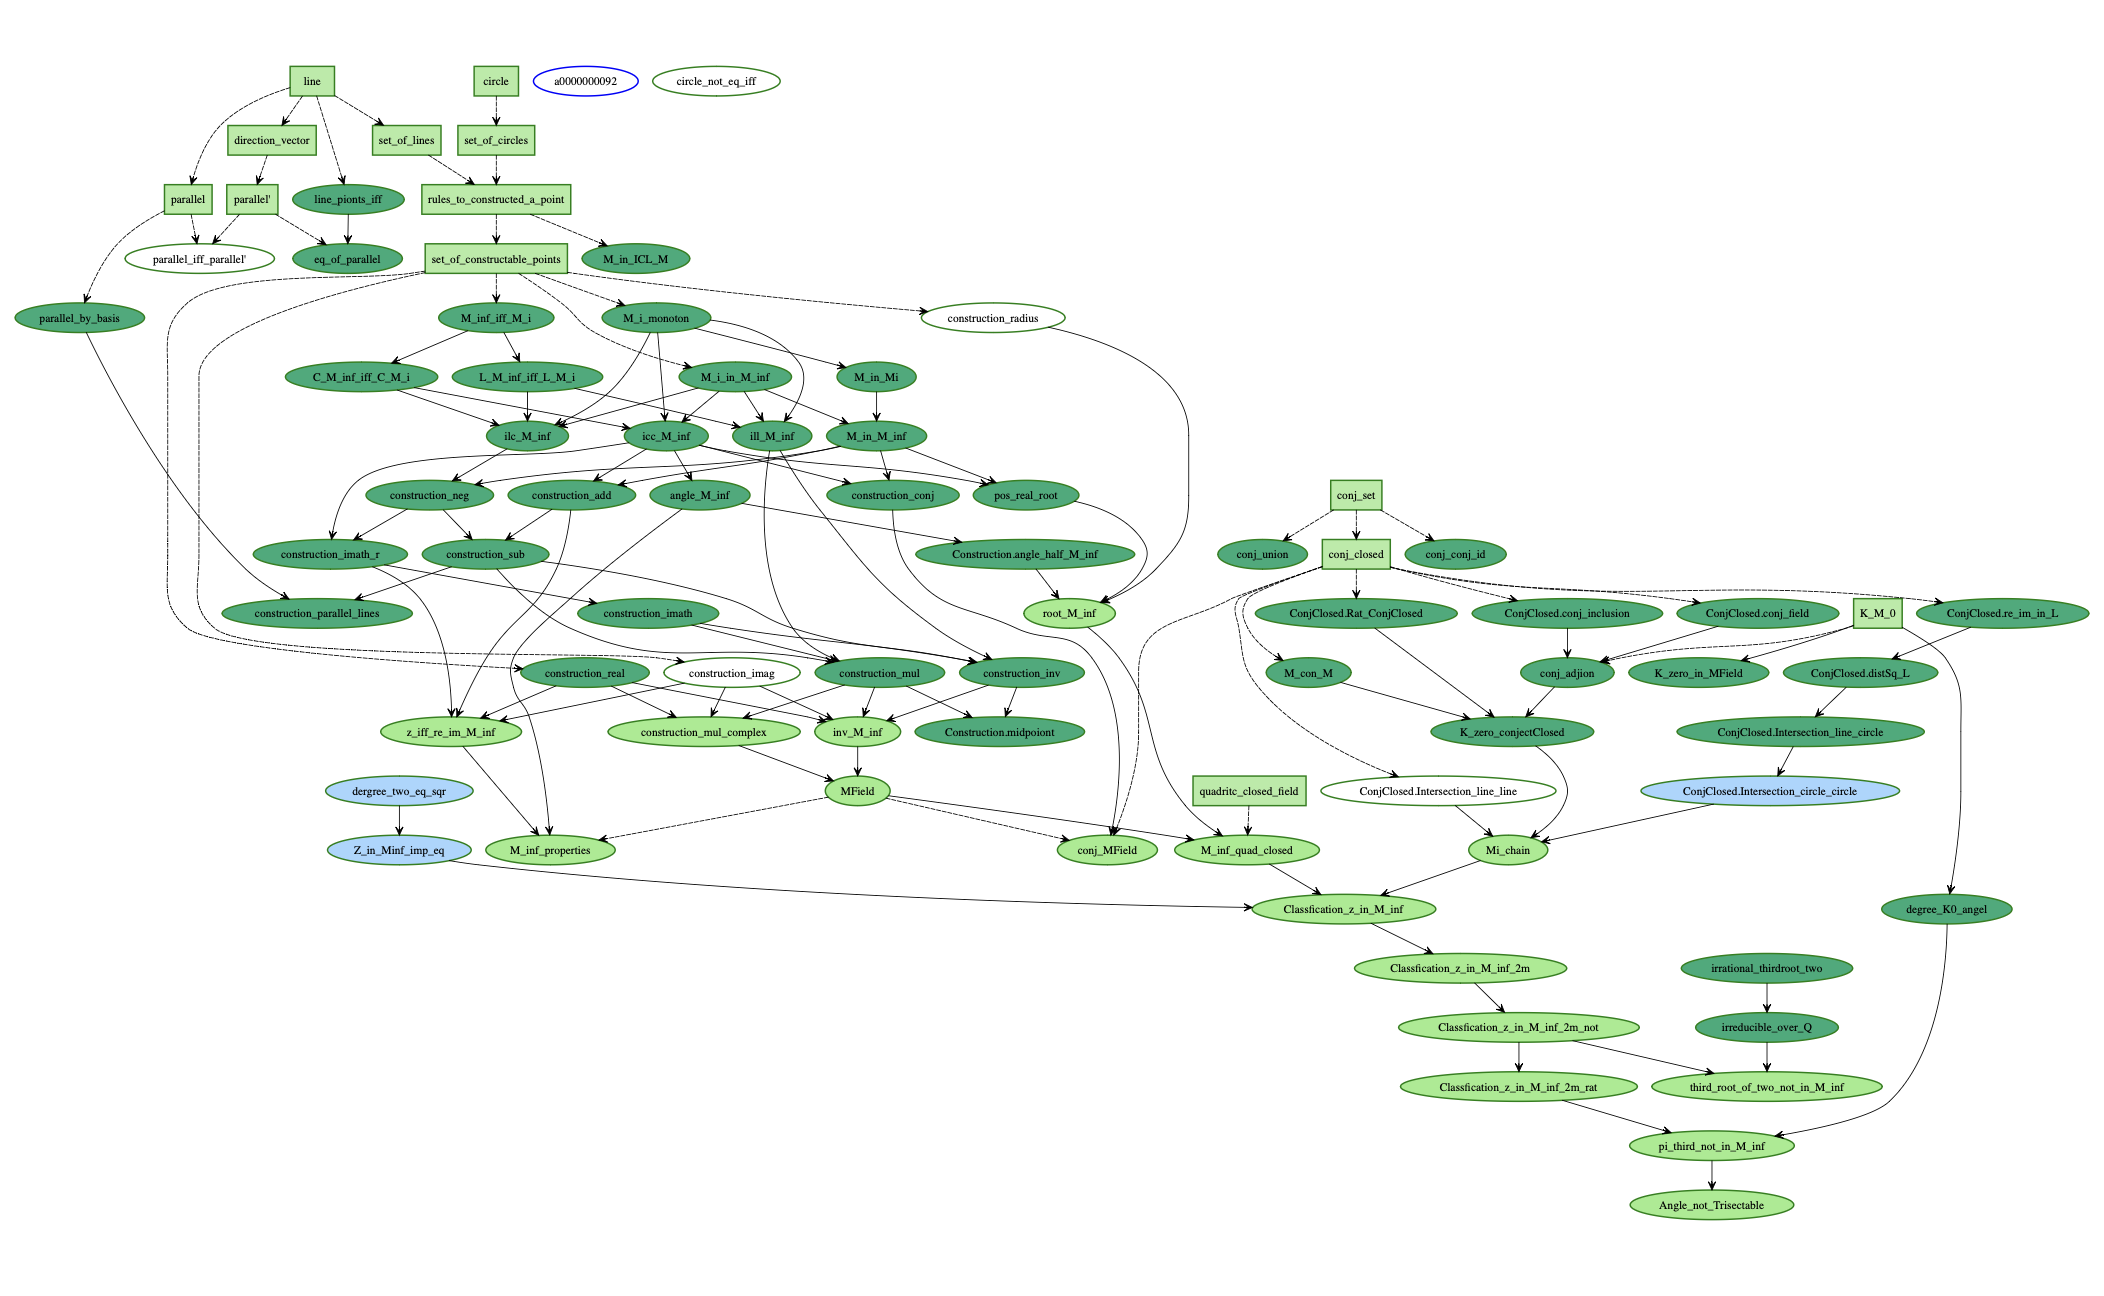
\includegraphics[angle=90, width=0.9\textwidth]{DependencyGraph}
    \label{fig:DependencyGraph}
    \caption{Dependency Graph}
\end{figure}
\clearpage
\section{A sample of Lean code}

\bibliographystyle{plainurl} % We choose the "plain" reference style
\bibliography{construct}



\nocite{*}
\end{document}